\documentclass[a4paper,oneside]{book}

\usepackage[english]{babel}
\usepackage[lined,boxed,commentsnumbered]{algorithm2e}
\usepackage[square,numbers]{natbib}
\usepackage[utf8]{inputenc}
\usepackage{a4wide}
\usepackage{amsbsy}
\usepackage{amsfonts}
\usepackage{amsmath}
\usepackage{amssymb}
\usepackage{amsthm}
\usepackage{array}
\usepackage{caption}
\usepackage{color}
\usepackage{enumerate}
\usepackage{epsfig}
\usepackage{fancyhdr}
\usepackage{float}
\usepackage{footnote}
\usepackage{geometry}
\usepackage{graphics}
\usepackage{graphicx}
\usepackage{hhline}
\usepackage{hyperref}
\usepackage{indentfirst}
\usepackage{lastpage}
\usepackage{latexsym}
\usepackage{layout}
\usepackage{listings}
\usepackage{lmodern}
\usepackage{multicol}
\usepackage{multirow}
\usepackage{pgfplots}
\usepackage{pictex}
\usepackage{pifont}
\usepackage{rotating}
\usepackage{scrextend}
\usepackage{setspace}
\usepackage{tabularx}
\usepackage{tikz-timing}[2014/10/29]
\usepackage{tikz}
\usepackage{tocloft}
\usepackage{verbatim}
\usepackage{wrapfig}
\usepackage{xcolor}
\usepackage{xparse}

\newcolumntype{P}[1]{>{\centering\arraybackslash}p{#1}}
\newcolumntype{M}[1]{>{\centering\arraybackslash}m{#1}}

\changefontsizes[12pt]{12pt}

\definecolor{lightgray}{gray}{0.9}

\bibliographystyle{ieeetr}

\setlength{\parindent}{2.5em}
\setlength{\parskip}{.5em}

\usetikztiminglibrary[rising arrows]{clockarrows}
\usetikzlibrary{arrows,backgrounds,patterns,snakes}
\usetikzlibrary{arrows,shapes.gates.logic.US,shapes.gates.logic.IEC,calc}

\hypersetup{urlcolor=blue,linkcolor=black,citecolor=black,colorlinks=true}

\newcommand{\PreserveBackslash}[1]{\let\temp=\\#1\let\\=\temp}
\newcolumntype{C}[1]{>{\PreserveBackslash\centering}p{#1}}
\newcolumntype{R}[1]{>{\PreserveBackslash\raggedleft}p{#1}}
\newcolumntype{L}[1]{>{\PreserveBackslash\raggedright}p{#1}}
\captionsetup[figure]{labelfont={small,bf},textfont={small,it},belowskip=-1pt,aboveskip=7pt}
% space remove between caption, figure, and text
\captionsetup[table]{labelfont={small,bf},textfont={small,it},belowskip=-1pt,aboveskip=7pt}
% space remove between caption, table, and text
\newcommand{\myarrow}[1][1cm]{\mathrel{%
		\vcenter{\hbox{\rule[-1.5\fontdimen8\textfont3]{#1}{\fontdimen8\textfont3}}}%
		\mkern-4mu\hbox{\usefont{U}{lasy}{m}{n}\symbol{41}}}}
\newcommand{\inlinecode}[2]{\colorbox{lightgray}{\lstinline[language=#1] $#2$}}
\newcommand{\dd}[1]{\mathrm{d}#1}
\renewcommand{\contentsname}{Table of Contents}
\renewcommand{\listfigurename}{List of Figures}
\renewcommand{\listtablename}{List of Tables}

% the following is needed for syntax highlighting
\fboxsep=3\fboxsep
\definecolor{dkgreen}{rgb}{0,0.6,0}
\definecolor{gray}{rgb}{0.5,0.5,0.5}
\definecolor{mauve}{rgb}{01,0,0.82}

\lstset{ %
    language=[Sharp]C,              % the language of the code
    basicstyle=\tt\footnotesize,    % the size of the fonts that are used for the code
    numbers=left,                   % where to put the line-numbers
    numberstyle=\tiny\color{gray},  % the style that is used for the line-numbers
    stepnumber=2,                   % the step between two line-numbers. If it's 1, each line
                                                                    % will be numbered
    numbersep=5pt,                  % how far the line-numbers are from the code
    backgroundcolor=\color{white},  % choose the background color. You must add \usepackage{color}
    showspaces=false,               % show spaces adding particular underscores
    showstringspaces=false,         % underline spaces within strings
    showtabs=false,                 % show tabs within strings adding particular underscores
    frame=single,                   % adds a frame around the code
    rulecolor=\color{black},        % if not set, the frame-color may be changed on line-breaks within not-black text (e.g. commens (green here))
    tabsize=2,                      % sets default tabsize to 2 spaces
    captionpos=b,                   % sets the caption-position to bottom
    breaklines=true,                % sets automatic line breaking
    breakatwhitespace=false,        % sets if automatic breaks should only happen at whitespace
    title=\lstname,                 % show the filename of files included with \lstinputlisting;
                                    % also try caption instead of title
    keywordstyle=\color{blue},      % keyword style
    commentstyle=\color{dkgreen},   % comment style
    stringstyle=\color{mauve},      % string literal style
    morekeywords={*, \ldots},       % if you want to add more keywords to the set
}


\newcommand*\colourcheck[1]{%
    \expandafter\newcommand\csname #1check\endcsname{\textcolor{#1}{\ding{51}}}%
}
\colourcheck{blue}
\colourcheck{green}
\colourcheck{red}

\NewDocumentCommand{\busref}{som}{\texttt{%
    #3%
    \IfValueTF{#2}{[#2]}{}%
    \IfBooleanTF{#1}{\#}{}%
}}

\hypersetup{urlcolor=blue,linkcolor=black,citecolor=black,colorlinks=true}

\addtolength{\oddsidemargin}{0.6cm}
\addtolength{\evensidemargin}{1.25cm}
\setlength{\headheight}{40pt}
\pagestyle{fancy}
\fancyhead{} % clear all header fields
\fancyhead[L]{
\begin{tabular}{rl}
    \begin{picture}(25,15)(0,0)
    \put(0,-8){
\includegraphics[width=8mm, height=8mm]{img/hcmut.png}}
    %\put(0,-8){\epsfig{width=10mm,figure=hcmut.eps}}
    \end{picture}&
	%
\includegraphics[width=8mm, height=8mm]{hcmut.png} & %
	\begin{tabular}{l}
		\textbf{\bf \ttfamily Ho Chi Minh University of Technology}\\
		\textbf{\bf \ttfamily Faculty of Computer Science and Engineering}
	\end{tabular}
\end{tabular}
}
\fancyhead[R]{
	\begin{tabular}{l}
		\tiny \bf \\
		\tiny \bf
	\end{tabular}  }
\fancyfoot{} % clear all footer fields

\fancyfoot[R]{\scriptsize \ttfamily Page {\thepage}/\pageref{LastPage}}
\renewcommand{\headrulewidth}{0.3pt}
\renewcommand{\footrulewidth}{0.3pt}
\renewcommand{\baselinestretch}{1.5}

\setcounter{secnumdepth}{4}
\setcounter{tocdepth}{3}
\makeatletter
\newcounter {subsubsubsection}[subsubsection]
\renewcommand\thesubsubsubsection{\thesubsubsection .\@alph\c@subsubsubsection}
\newcommand\subsubsubsection{\@startsection{subsubsubsection}{4}{\z@}%
                                    {-3.25ex\@plus -1ex \@minus -.2ex}%
                                    {1.5ex \@plus .2ex}%
                                    {\normalfont\normalsize\bfseries}}
\newcommand*\l@subsubsubsection{\@dottedtocline{3}{10.0em}{4.1em}}
\newcommand*{\subsubsubsectionmark}[1]{}
\makeatother

\newcommand{\fancyfootnotetext}[2]{%
    \fancypagestyle{dingens}{%
    \fancyfoot[LO,RE]{\parbox{12cm}{\footnotemark[#1]\footnotesize #2}}%
    }%
    \thispagestyle{dingens}%
}

\newcommand{\listhistogramname}{\large{List of chart}}
\newlistof{histogram}{exp}{\listhistogramname}
\newcommand{\histogram}[1]{%
\refstepcounter{histogram}
\par\noindent\textbf{Histogram \thehistogram. #1}
\addcontentsline{exp}{histogram}
{\protect\numberline{\thehistogram}#1}\par}

\begin{document}

\begin{titlepage}
\thispagestyle{empty}
\usetikzlibrary{calc}
\begin{tikzpicture}[overlay,remember picture]
    \draw [line width=3pt]
        ($ (current page.north west) + (2.0cm,-2.0cm) $)
        rectangle
        ($ (current page.south east) + (-1.5cm,1.8cm) $);
    \draw [line width=1pt]
        ($ (current page.north west) + (2.15cm,-2.15cm) $)
        rectangle
        ($ (current page.south east) + (-1.65cm,1.95cm) $);
\end{tikzpicture}

\begin{center}
	\begin{large}
        {\fontsize{12pt}{1}\textbf{VIETNAM NATIONAL UNIVERSITY HO CHI MINH CITY}} \\
		\textbf{HO CHI MINH UNIVERSITY OF TECHNOLOGY} \\
		\textbf{Faculty of Computer Science and Engineering}
	\end{large} \\
	\textbf{--------------------  *  ---------------------}\\

	\vspace{0.8cm}
	
\includegraphics[scale=.35]{img/hcmut.png}\\
	\vspace{0.8cm}
    {\fontsize{14.4pt}{1}\selectfont \textbf{TANG QUOC THAI}}\\[.75cm]
	\vspace{0.8cm}
	{\fontsize{14.4pt}{1}\selectfont \textbf{Internship 2 Report}}\\[.75cm]
	{\fontsize{17pt}{1}\selectfont \textbf{\MakeUppercase{APPLICATION OF LARGE LANGUAGE MODELS IN SOFTWARE ERROR DEBUGGING}}}
\end{center}
\vspace{4cm}

\hspace{.5cm}
\begin{center}
    {\fontsize{15pt}{1} Ho Chi Minh City, January 2024}
\end{center}
\end{titlepage}
\newpage

\begin{titlepage}
\thispagestyle{empty}
\usetikzlibrary{calc}
\begin{tikzpicture}[overlay,remember picture]
    \draw [line width=3pt]
        ($ (current page.north west) + (2.0cm,-2.0cm) $)
        rectangle
        ($ (current page.south east) + (-1.5cm,1.8cm) $);
    \draw [line width=1pt]
        ($ (current page.north west) + (2.15cm,-2.15cm) $)
        rectangle
        ($ (current page.south east) + (-1.65cm,1.95cm) $);
\end{tikzpicture}

\begin{center}
	\begin{large}
		{\fontsize{12pt}{1}\textbf{VIETNAM NATIONAL UNIVERSITY HO CHI MINH CITY}}
		\textbf{HO CHI MINH UNIVERSITY OF TECHNOLOGY} \\
		\textbf{Faculty of Computer Science and Engineering}
	\end{large} \\
	\textbf{--------------------  *  ---------------------}\\

	\vspace{0.8cm}
	
\includegraphics[scale=.35]{img/hcmut.png}\\
	\vspace{0.8cm}
	{\fontsize{14.4pt}{1}\selectfont \textbf{TANG QUOC THAI}}\\[.75cm]
	\vspace{0.8cm}
	{\fontsize{14.4pt}{1}\selectfont \textbf{Internship 2 Report}}\\[.75cm]
	{\fontsize{17pt}{1}\selectfont \textbf{\MakeUppercase{APPLICATION OF LARGE LANGUAGE MODELS IN SOFTWARE ERROR DEBUGGING}}}
\end{center}
\vspace{.4cm}

\begin{center}
	{\fontsize{14.4pt}{1} MAJOR: COMPUTER SCIENCE}\\[.2cm]
    {\fontsize{14.4pt}{1}
    \textbf{INSTRUCTOR:}\\[.2cm]
    \textbf{Assoc. Prof. QUAN THANH THO}\\[.2cm]
    {\fontsize{14.4pt}{1} Ho Chi Minh City, January 2024}}
\end{center}
\end{titlepage}

\newpage
\begin{titlepage}
\thispagestyle{empty}
\begin{center}
    \begin{large}
        \textbf{Internship 2 Signature Page}
    \end{large}
\end{center}
\vspace{1.2cm}
\begin{itemize}
    \item[] \textbf{Project Title:} Application of Large Language Models in Software Error Debugging
    \vspace{1cm}

    The Internship 2 Report is submitted in partial fulfillment of the requirements for the degree of Master of Science in Computer Science.
    \vspace{2cm}

    \begin{minipage}{0.5\textwidth}
        \textbf{Student:} \\[2cm]
        Tang Quoc Thai\\[0.25cm]
        \hrulefill
        \rule{7cm}{0.4pt}
    \end{minipage}
    \begin{minipage}{0.5\textwidth}
        \begin{flushright}
            \textbf{Instructor:} \\[2cm]
            Assoc. Prof. Quan Thanh Tho\\[0.25cm]
            \hrulefill
            \rule{7cm}{0.4pt}
        \end{flushright}
    \end{minipage}
    \vspace{1cm}
\end{itemize}
\end{titlepage}

\newpage
\tableofcontents

\newpage
\listoffigures

\newpage
\listoftables

\newpage
\chapter{Topic Introduction}

\section{General Introduction}
In recent years, generative AI models, particularly Large Language Models (LLMs), have garnered significant attention from both the Artificial Intelligence (AI) research community and the general public. These models exhibit a remarkable capacity to address a diverse array of intricate language-based tasks. Their advancements are propelled by factors such as increased model parameter count, augmented training data volume, and refined training configurations~\cite{brown2020language, radford2019language, hernandez2021scaling, kaplan2020scaling}. Prominent LLMs like LaMDA~\cite{thoppilan2022lamda} and GPT-4~\cite{openai2023gpt4} demonstrate exceptional proficiency in applications ranging from translation and classification to creative writing and code generation. Such capabilities, previously necessitating task-specific models developed by domain experts using specialized data, are now achieved by these broad, state-of-the-art LLMs.

Concurrently, researchers have enhanced the steerability, reliability, and utility of these models through techniques like fine-tuning and reinforcement learning with human feedback~\cite{ouyang2022training, bai2022training}. These advancements empower models to better understand user intent, thereby enhancing user-friendliness and practicality. Recent studies also showcase LLMs' potential to program and control other digital tools, such as APIs, search engines, and even fellow generative AI systems~\cite{schick2023toolformer, mialon2023augmented}. This integration of individual components facilitates improved utility, performance, and generalization. At the forefront of these trends, there lies a prospect where LLMs can potentially execute any task traditionally performed at a computer.

While generative AI models have primarily been deployed as modular specialists for tasks like image generation from captions or text transcription from speech, the focus is on viewing LLMs as versatile building blocks for creating additional tools. The development and integration of these tools into systems may necessitate time and significant reconfiguration of existing processes across diverse industries. Nevertheless, early adoption trends are already emerging. Despite their limitations, LLMs are increasingly finding integration into specialized applications in areas such as writing assistance, coding, and legal research. These specialized applications enable businesses and individuals to incorporate LLMs into their existing workflows.

The emphasis is on the significance of these complementary technologies, particularly because standalone general-purpose LLMs may still exhibit unreliability for certain tasks, attributable to issues such as factual inaccuracies, inherent biases, privacy concerns, and risks associated with disinformation~\cite{abid2021persistent, schramowski2022large, goldstein2023generative}. However, specialized workflows, encompassing tooling, software, or human-in-the-loop systems, can effectively mitigate these shortcomings by incorporating domain-specific expertise. For instance, Casetext provides LLM-based legal research tools that furnish lawyers with quicker and more accurate legal research results, utilizing embeddings and summarization to counteract the risk of GPT-4 potentially providing inaccurate details about a legal case or set of documents. GitHub Copilot, a coding assistant, leverages LLMs to generate code snippets and auto-complete code, allowing users to accept or reject suggestions based on their expertise. In essence, while GPT-4, on its own, might not inherently `know what time it is,' incorporating a watch can address this limitation.

Moreover, a positive feedback loop may emerge as LLMs surpass specific performance thresholds, enabling them to contribute to the development of tools that enhance their usefulness and usability across diverse contexts. This could potentially reduce the cost and engineering expertise required to create such tools, thereby accelerating LLMs adoption and integration~\cite{chen2021evaluating, peng2023impact}. LLMs may also become valuable assets in machine learning model development—serving as coding assistants for developers.

In a recent study~\cite{peng2023impact}, a cumulative total of 166 offers were distributed as part of the experiment, and 95 of these offers were accepted. The 95 developers underwent random assignment into control and treated groups, with 45 individuals in the treated group and 50 in the control group. Thirty-five developers from both the treated and control groups effectively completed the designated task and the subsequent survey.

\begin{figure}[H]
    \centering
    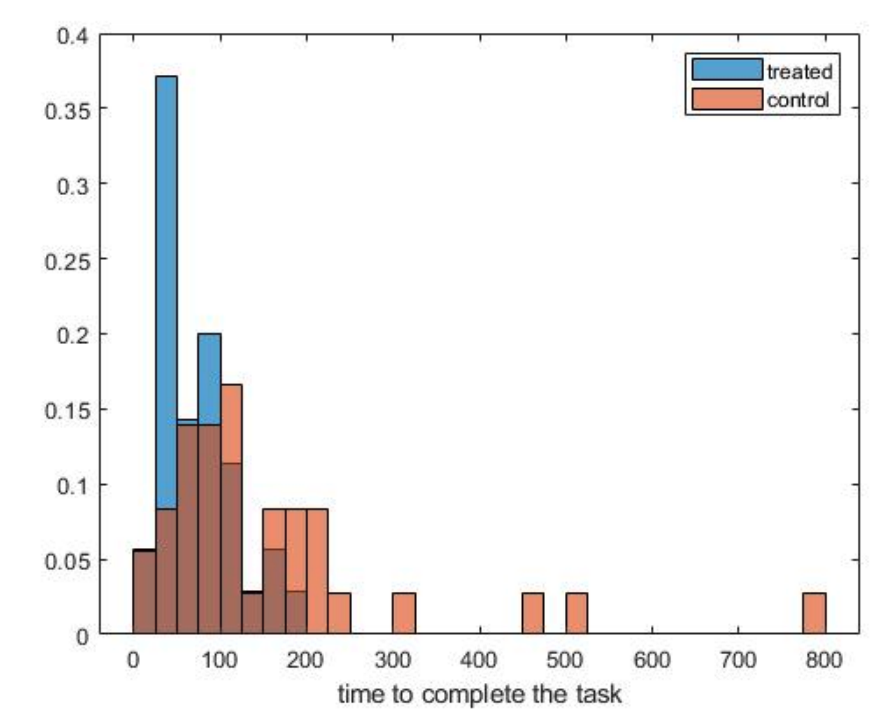
\includegraphics[width=0.5\textwidth]{img/task_completion_time.png}
    \caption{Distribution of time to completion between treated and control groups~\cite{peng2023impact}.}\label{fig:task_completion_time}
\end{figure}

Figure~\ref{fig:task_completion_time} illustrates the distribution of time to completion between the treated and control groups. When conditioned on task completion, the average completion time for the treated group is 71.17 minutes, compared to 160.89 minutes for the control group, resulting in a \boldmath{$55.8\%$}~\textbf{reduction in completion time}.

\section{Self-Correcting LLMs for Software Development}
\begin{figure}[H]
    \centering
    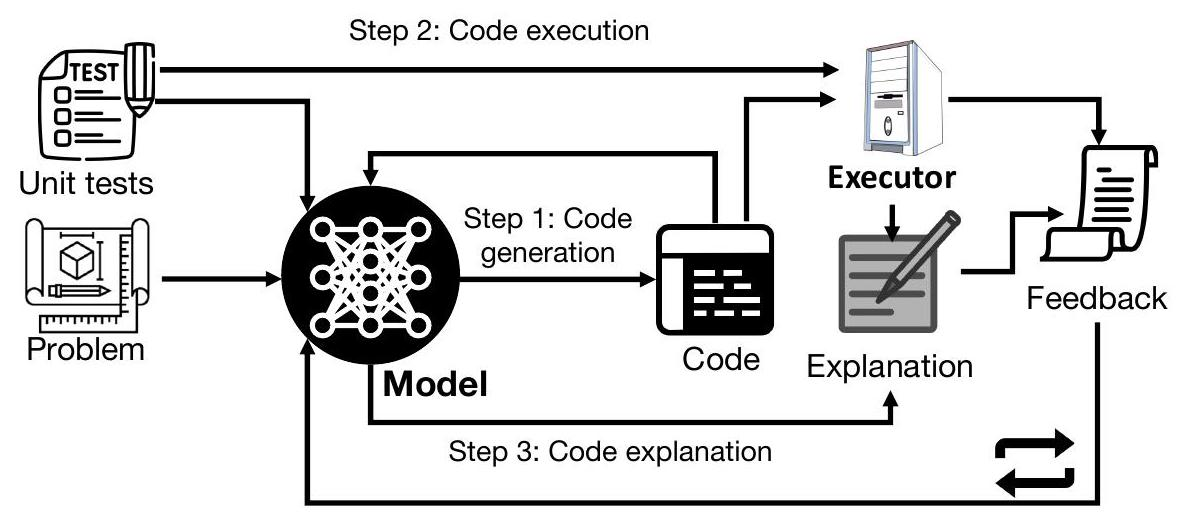
\includegraphics[width=0.90\textwidth]{img/self_debug.jpg}
    \caption{
        A prevalent approach for iterative debugging employing a large language model involves multiple steps~\cite{chen2023teaching}.}\label{fig:self_debug}
\end{figure}

Figure~\ref{fig:self_debug} depicts a typical scenario involving the application of self-correcting LLMs for iterative debugging, employing a pretrained large language model without undergoing finetuning.

A single iteration within this framework comprises three sequential steps: Generation, Explanation, and Feedback.

\begin{itemize}
    \item In the Generation step, the model predicts candidate programs based on the given problem description.

    \item Throughout the Explanation step, the model is prompted to process the predictions in a semantically meaningful manner. This may involve explaining the prediction in natural language or creating an execution trace of the predicted code for a sample input.

    \item For the Feedback step, a feedback message evaluating the correctness of the predicted code is generated. This assessment can be obtained by querying the model itself or externally generating feedback from unit tests.
\end{itemize}

The debugging process concludes either when the feedback message confirms the correctness of the prediction or when the maximum allowed number of debugging turns is reached.

\textbf{Simple feedback}: a straightforward form of automatic feedback is a sentence indicating code correctness without additional detailed information, omitting the Explanation step in a complete Self-Debugging turn. For example, in text-to-SQL generation, the few-shot prompt issues the feedback message `The SQL prediction above is correct' for accurate SQL queries and `The SQL prediction above is wrong. Please fix the SQL' for incorrect predictions.

\textbf{Unit test feedback}: is applicable to code generation tasks where the problem description includes unit tests. In addition to using code execution to assess correctness, feedback can incorporate execution results, providing richer debugging information. Intuitively, examining runtime errors and execution results of failed unit tests enhances the effectiveness of human programmers in debugging. Our experiments will illustrate that leveraging unit tests whenever available consistently enhances the performance of self-correcting LLMs.

\textbf{Code explanation feedback}: remains an unexplored area in the context of model-generated feedback on code generation. Despite the promising progress demonstrated by large language models in generating critiques to avoid harmful model outputs and improving performance on certain natural language tasks, the effectiveness of such feedback on code generation tasks has not been established in prior work. Conversely, large language models have exhibited proficiency in describing their generated problem solutions in both textual and code formats.

\textbf{Execution trace feedback}: extends beyond explaining the code itself, as human programmers often comprehend the semantic meaning of code through simulating the execution process. Previous work on code repair has indicated that training repair models on execution traces enhances debugging performance. Thus, when unit tests are available, an alternative explanation feedback format is examined, wherein the LLMs explains the intermediate execution steps line-by-line. It is noteworthy that both the execution trace and the line-by-line explanation originate from model generation rather than code execution. Therefore, trace feedback does not necessitate more information than pure code explanation feedback, specifically no access to intermediate execution states.

\section{Research Objectives}
TBD

\section{Research Scopes}
TBD

\chapter{Related Works}

\section{A Taxonomy for Self-Correcting LLMs with Automated Feedback}
For the sake of clean exposition, this research first presents a conceptual framework outlining the overall process of correcting LLMs with feedback, thereby establishing the scope. It then proceeds to identify five primary dimensions that serve as classification criteria for existing works: 1. What gets corrected, 2. What is the source of the feedback, 3. What is the format of the feedback, 4. When the feedback is used, and 5. How to correct the model with feedback.

\subsection{Conceptual Framework}
The general process of correcting LLMs with automated feedback is formulated in Figure~\ref{fig:taxonomy}, using an analogy of medical treatment in daily life. Three parties are involved in this process:

\begin{itemize}
    \item Language Model (Patient). A language model $\mathcal{M}: \mathcal{X} \rightarrow \mathcal{Y}$ performs a specific task by mapping an input $x \in \mathcal{X}$ to an output text $\hat{y} \in \mathcal{Y}$. This formulation encompasses a wide range of NLP tasks. For example, in summarization, $x$ is a passage, $\hat{y}$ is the generated summary; for question-answering, $x$ is a question and $\hat{y}$ is the predicted answer. The initial generation $\hat{y}$ may be imperfect and suffer from various problems such as hallucination and incorrect reasoning.

    \item Critic Model (Doctor \& Diagnosis). A critic model $\mathcal{C}: \mathcal{X} \times \mathcal{Y} \rightarrow \mathcal{F}$ learns to generate feedback $x, \hat{y} \rightarrow c$ where $\hat{y} \sim \mathcal{M}(x)$ is the output or partial output of the language model, and $c$ is the feedback of some format, e.g., scalar value, or natural language. A simple example is binary feedback of whether the output is good or bad given the input $(\mathcal{C}: \mathcal{X} \times \mathcal{Y} \rightarrow\{0,1\})$.

    \item Refine Model (Treatment). A refine model $\mathcal{R}$: $\mathcal{X} \times \mathcal{Y} \times \mathcal{F} \rightarrow \mathcal{Y}$ learns to repair an output $x, \hat{y}, c \rightarrow$ $y_{\text {new }}$ based on the feedback $c$, where $y_{\text {new }}$ is the revised output. Besides repairing output, some refine models directly repair the language model $\mathcal{M}$ through fine-tuning or reinforcement learning.
\end{itemize}

Based on the above formulation, Figure~\ref{fig:taxonomy} illustrates the fundamental interaction among the language model $\mathcal{M}$, the critic model $\mathcal{C}$, and the refine model $\mathcal{R}$. However, the specific model design in existing works varies along five crucial axes, which this research will elaborate on in the following sections.

\begin{itemize}
    \item \textbf{Hallucination}: An open challenge for LLMs is that they often hallucinate by making up facts or citing sources that do not exist~\cite{li2023halueval, zhang2023language}. These hallucinated contents are often quite plausible-sounding, making it difficult even for humans to detect~\cite{clark2021thats}. To address this, several studies have proposed the collection of automated feedback on potential factual inaccuracies by cross-referencing the output generated by the model with credible knowledge sources. The gathered feedback can then be utilized by a subsequent refinement model to correct hallucinations~\cite{gao2023rarr, zhang2023language}.

    \item \textbf{Unfaithful Reasoning}: LLMs have exhibited a strong ability in solving complex reasoning tasks with improved reasoning strategies, such as Chain-of-Thought prompting~\cite{wei2023chainofthought}. However, recent studies~\cite{golovneva2023roscoe,ribeiro2023street,lyu2023faithful} found that LLMs occasionally make unfaithful reasoning, i.e., the derived conclusion does not follow the previously generated reasoning chain. To address this, existing works have proposed the use of automated feedback from external tools or models for guiding the reasoning process~\cite{xie2023selfevaluation, yao2023tree}, verifying the reasoning process and rectifying errors~\cite{he2022rethinking,pan2023logiclm}, or finetuning LLMs with process-based feedback~\cite{huang2022large, lightman2023lets}.

    \item \textbf{Toxic, Biased, and Harmful Contents}: LLMs have been observed to occasionally generate content that is toxic, biased, or harmful due to biases present in the training data~\cite{shaikh-etal-2023-second}. To rectify this, reinforcement learning from human feedback (RLHF)~\cite{ouyang2022training, bai2022training} has been extensively employed to train LLMs to align more closely with human values, such as being helpful, honest, and harmless. However, RLHF is heavily dependent on highquality human feedback, the collection of which can be resource-intensive. To alleviate this, recent works~\cite{lu2022quark, gou2023critic} have also explored collecting automated feedback to identify and correct potentially harmful outputs.

    \item \textbf{Flawed Code}: Besides generating natural language text, LLMs also show strong abilities to generate computer programs (i.e., code)~\cite{chen2022codet}. However, the generated code can sometimes be flawed or incorrect. To fix this, the approach of learning from automated feedback has been extensively applied in code generation~\cite{chen2023teaching, olausson2023selfrepair}, largely facilitated by the ease of obtaining such feedback through the execution of generated code with the corresponding compilers or interpreters.
\end{itemize}

\begin{figure}[H]
    \centering
    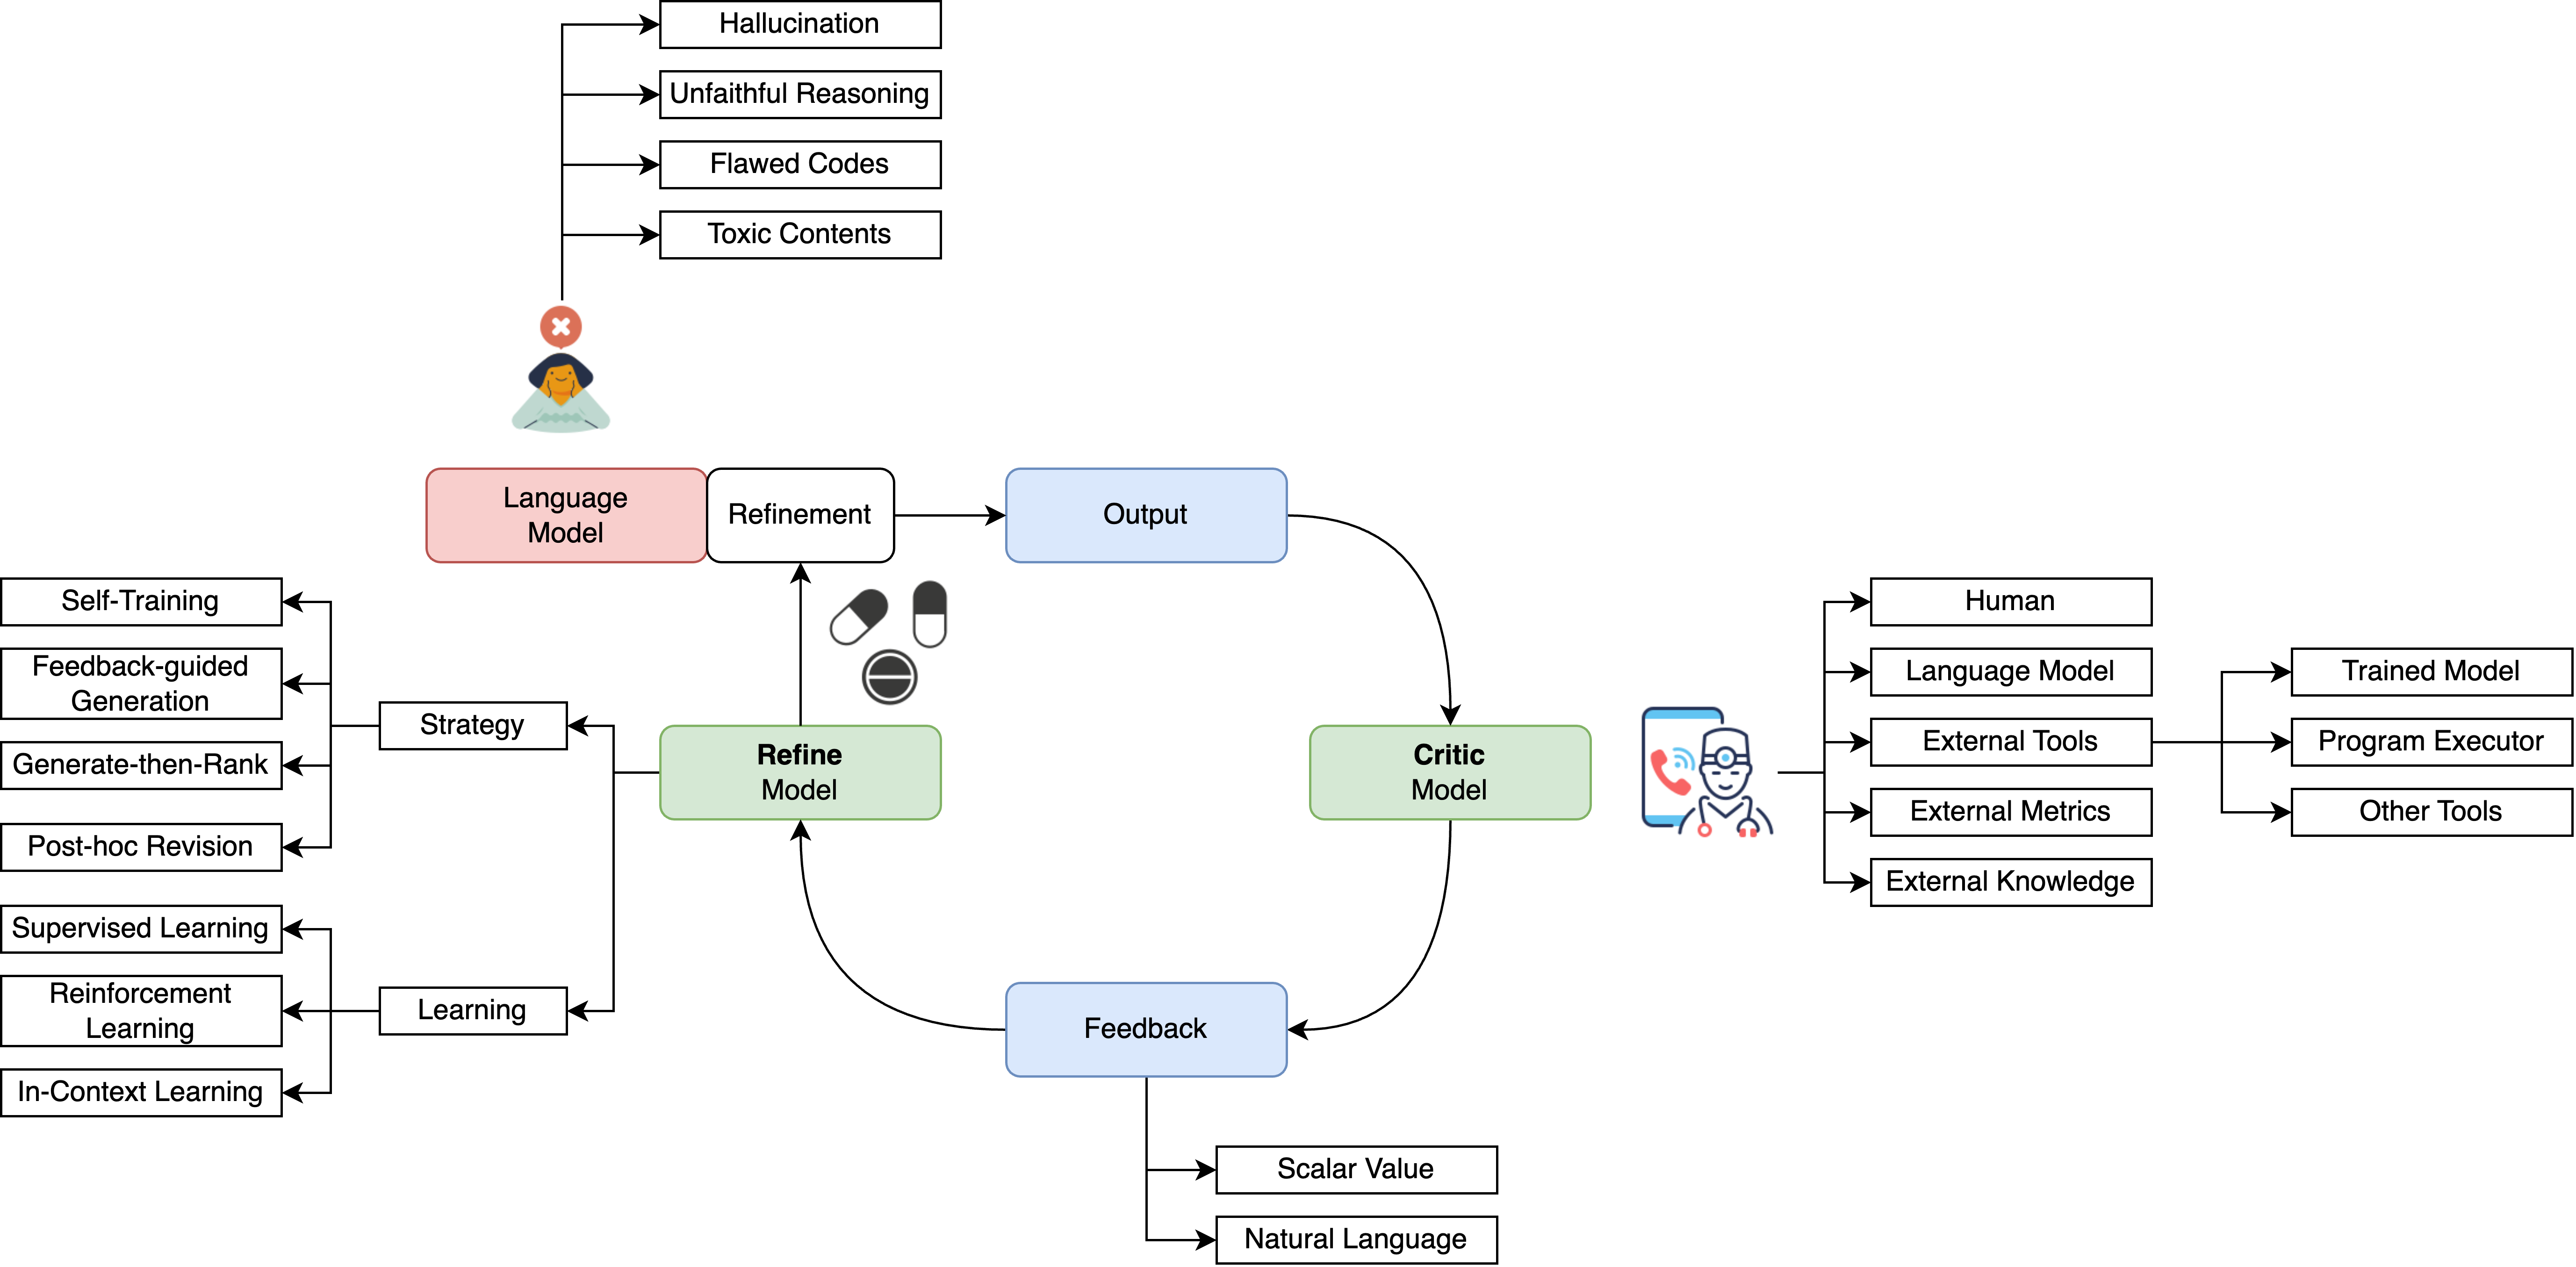
\includegraphics[width=0.90\textwidth]{img/taxonomy.png}
    \caption{A conceptual framework for self-correcting LLMs with automated feedback.}\label{fig:taxonomy}
\end{figure}

\subsection{What is the source of the feedback?}
Feedback can be broadly divided into two categories: human feedback and automated feedback. Fernandes et al.~\cite{fernandes2023bridging} provided a survey on integrating human feedback for language generation. This research focuses on the emerging research area of automated feedback, which explores the possibility of LLMs to self-correct without constant human intervention. Automated feedback typically originates from two sources, distinguished by their relationship with the LLMs: self-feedback (i.e., the feedback originates from the LLMs itself) and external feedback (i.e., the feedback is derived from external models, tools, or knowledge sources).

\begin{itemize}
    \item \textbf{Self-Feedback}: The LLMs itself can be utilized as a feedback provider. One straightforward way is to directly evaluate the quality of the generated outputs through prompting and subsequently use this feedback to refine the results~\cite{madaan2023selfrefine, shinn2023reflexion}. This process can be iterative, with the model continually refining its output until it meets a certain standard. This continuous self-improvement strategy has been found particularly useful by numerous studies~\cite{selfee2023, yan-etal-2023-learning}, especially in scenarios where external feedback is unavailable or limited.

    \item \textbf{External Feedback}: Feedback can originate from sources external to the LLMs, typically including (1) other trained models~\cite{yan-etal-2023-learning, lightman2023lets}, (2) external tools~\cite{gou2023critic, charalambous2023new}, (3) external knowledge sources~\cite{gao2023rarr, yu2023improving}, and (4) external evaluation metrics~\cite{jung-etal-2022-maieutic, welleck2022generating}. External feedback provides a valuable outside perspective which is particularly useful in identifying errors that the LLMs might not recognize on its own. For example, code interpreters are widely used in programming tasks to provide real-time error messages; while external knowledge sources can be utilized to verify the factual accuracy of the LLMs' output.
\end{itemize}

\subsection{What is the format of the feedback?}
The selection of feedback format requires the consideration of its expressivity, the ease of its collection, and its potential to improve systems~\cite{fernandes2023bridging}. In existing works, automated feedback is typically in the form of a scalar value signal or in natural language.

\begin{itemize}
    \item \textbf{Scalar Value Feedback}: In this scenario, the critic model maps the input and output to a single score $(\mathcal{C}: \mathcal{X} \times \mathcal{Y} \rightarrow \mathcal{N} \subseteq \mathbb{R})$. Scalar value feedback can be easily integrated into the training/decoding process of LLMs. For example, SelfVerification~\cite{weng2023large} ranks candidate outputs to find the optimal one based on the realvalue feedback score assigned by the critic model to each candidate. Similarly, Xie et al.~\cite{xie2023selfevaluation} use real-value feedback for each intermediate reasoning step to guide the model in performing a stochastic beam search for the optimal solution. However, despite its flexibility, scalar value feedback is often less informative to capture detailed information necessary for model correction.

    \item \textbf{Natural Language Feedback}: Natural language feedback offers greater expressivity than scalar value feedback, providing richer information that can highlight the shortcomings of the current output or suggest specific improvements. This form of feedback is particularly crucial for certain applications, such as text editing and code generation. For text editing, PEER~\cite{schick2022peer} trains an LLMs to generate detailed suggestions for edits to the initial generated text, such as `remove unsourced claim' or `rewrote the guacamole question for clarity'. For code generation, SelfDebug~\cite{chen2023teaching} uses LLMs to generate explanations for the produced code and utilize both the explanation and the execution results as feedback to enhance coding solutions.
\end{itemize}

\subsection{When to correct the model with feedback?}
Depending on the timing of using automated feedback to correct the model, existing works can be divided into three major categories:

\begin{itemize}
    \item \textbf{Training-time Correction}: The ideal scenario is to rectify a flawed model during training, prior to its deployment for use. Once feedback has been collected, it is directly used to optimize the model parameters. Human feedback is typically used for training-time correction, as exemplified by the widely adopted RLHF approach~\cite{ouyang2022training}. For leveraging automated feedback, a common strategy is self-training~\cite{huang2022large}, where the model is trained with its own generated high-quality output filtered by the critic model. While training-time correction is a pre-hoc strategy that addresses problems during training, its practical application may be hindered by: (1) the infeasibility of fine-tuning closed-source LLMs like GPT-4~\cite{openai2023gpt4}, (2) the potential unavailability of feedback during model training, and (3) the requirement for the feedback to be `optimizable', e.g., a numerical score serving as the basis for model optimization.

    \item \textbf{Generation-time Correction}: This strategy utilizes automated feedback to guide the language model during generation, allowing the model to correct errors in its outputs as it is being generated. For example, for proof generation, several works utilize the automated feedback of the intermediate reasoning steps to guide the model to recover from incorrect generation and search for the optimal solution more efficiently~\cite{yang-etal-2022-generating, lightman2023lets}.

    \item \textbf{Post-hoc Correction}: Finally, post-hoc correction involves refining the model output after it has been generated, without updating the model parameters. This typically involves iteratively generating output, receiving feedback, and refining output. Post-hoc correction provides more flexibility than the previous two strategies as it does not require training the LLMs or accessing its parameters. Furthermore, post-hoc correction enhances explainability as it facilitates incorporating more informative natural language feedback. This allows for a more transparent visualization and interpretation of the self-correction process.
\end{itemize}

\subsection{How to correct the model with feedback?}
Various concrete strategies have been proposed to correct LLMs with automated feedback, tailored to the different dimensions mentioned in previous sections. For example, self-training is often used for training-time correction. Generate-then-rank often comes with scalar value feedback. Self-refine is the strategy that uses the same LLMs as both the critic model and the refine model.

Building upon the taxonomy established in the preceding sections, existing works on correcting LLMs with (automated) feedback are collated in Table 1 and Table 2 based on two major selection criteria:

\begin{enumerate}
    \item \textbf{Automated Feedback}: Explicit feedback is involved to assess the quality of the model output, focusing on automated feedback originating from external models, metrics, knowledge, etc. However, some representative works of human feedback are covered for completeness.

    \item \textbf{Model Refinement}: The feedback acts as a directive to enhance the LLMs, either by: (1) updating model parameters, or (2) altering the model's output during or after the generation process.
\end{enumerate}

\section{Training-Time Correction}
This section delves into methodologies that rectify model behavior during the training phase. Three typical strategies for training-time correction are identified, each utilizing different forms of feedback to modify the model parameters during training: human feedback, a reward model approximating human feedback, and automated feedback.

\subsection{Learning from Human Feedback}
The next-word prediction objective of LLMs pretraining is not inherently designed to encapsulate human values or preferences. This misalignment can lead to unintended consequences like generating harmful, misleading, or biased content~\cite{kenton2021alignment}. Many research efforts have explored integrating human feedback to better align LLMs with human values and expectations.Wang~\cite{wang2023aligning} and Fernandes~\cite{fernandes2023bridging} extensively reviewed this area. However, this research focuses on automated feedback, so only representative works in this direction are touched upon.

\textbf{Direct Optimization with Human Feedback}: In an ideal scenario, human feedback would directly optimize model parameters. Typically, this approach follows: (1) LLMs generate candidate outputs, (2) Humans provide feedback or refinements on these outputs, and (3) LLMs are optimized on the collected (outputs, feedback) to align with human preferences. One strategy is fine-tuning the model on outputs with positively-labeled feedback. For example, Sparrow~\cite{glaese2022improving} fine-tunes LLMs on dialogues rated as preferred and rule compliant (concerning correctness, harmfulness, and helpfulness) by humans. Similarly, Scheurer~\cite{scheurer2023training} uses an LLMs to generate refinements of the original output based on human feedback, and fine-tunes the original LLMs on the best refinement. A similar idea is adopted to fine-tune code generation models~\cite{chen2023improving}. First, human annotators provide feedback for incorrect codes. A refinement model utilizes this to correct the code. Finally, the refined code fine-tunes the code-generating LLM. However, using only positive data (human-refined or positive-rated) may constrain identifying and correcting negative attributes or errors. Chain-of-Hindsight~\cite{liu2023chain} addresses this by fine-tuning the LLMs on outputs paired with both positive and negative feedback. Beyond fine-tuning, other optimization methods are explored. For example, Gao et al.~\cite{gao2023continually} uses human feedback as the reward signal and optimizes the model with contextual bandit learning.

\textbf{Reward Modeling and RLHF}: Employing human feedback directly may not always be practical since collecting it can be labor-intensive and time-consuming. An efficient alternative is training a reward model that emulates human feedback. Once trained, this can provide consistent, real-time feedback for every output, circumventing constant human involvement. A prominent example is Reinforcement Learning from Human Feedback (RLHF)~\cite{ouyang2022training}. It first has humans label preference for different LLMs outputs and trains the reward model to predict human preference. Then reinforcement learning algorithms (e.g., Proximal Policy Optimization (PPO)~\cite{schulman2017proximal}) optimize the model. RLHF and variants have proven effective in making LLMs more beneficial and less harmful~\cite{bai2022training}, and instilling moral correctness~\cite{ganguli2023capacity}.

\subsection{Learning with Automated Feedback}
Given the resource-intensive nature of collecting human feedback, multiple studies have investigated the utilization of automated feedback to reduce the dependence on human intervention. To distinguish between human and automated feedback, human feedback is defined as a quality assessment conducted by human evaluators on outputs generated by the base model. In contrast, automated feedback is acquired in an offline environment without human assessment of model outputs. This discussion primarily addresses training-time strategies employing two types of automated feedback: extrinsic feedback from external metrics/models and intrinsic feedback from the language model itself.

\textbf{External Metric Guidance}: Feedback from external metrics is commonly employed for training-time correction. Due to the discrete nature of metric signals, most approaches focus on non-differentiable training techniques. Minimum Risk Training~\cite{shen-etal-2016-minimum} optimizes model parameters with external evaluation metrics~\cite{xu-etal-2022-errors, xu-etal-2023-sescore2} by incorporating metric scores with maximum log-likelihood in the loss function. This method can optimize metric scores during training. However, it may lead to robustness deficiencies in some metrics~\cite{yan-etal-2023-bleurt}, such as BLEURT~\cite{sellam-etal-2020-bleurt}. Liu et al.~\cite{liu-liu-2021-simcls} leverages a contrastive learning framework to rerank candidates based on metric scores, bridging the gap between training and inference objectives. Li et al.~\cite{li-etal-2019-deep} employ a deep Reinforcement Learning (RL) algorithm, and~\cite{jauregi-unanue-etal-2021-berttune} leverage Gumbel softmax~\cite{jang2017categorical} to build distributional semantic reward from BERTScore~\cite{zhang2020bertscore} and mitigate exposure bias. To stabilize gradients, Wu et al.~\cite{wu2021textgail} uses a contrastive discriminator and PPO to imitate human texts. Recently, Chang et al.~\cite{chang2023learning} propose a more efficient RL algorithm, RLGF, than PPO~\cite{schulman2017proximal} to finetune LLMs with pre-defined reward. They integrate a reasonable but incomplete guide policy into a policy gradient framework and learn a near-optimal strategy. Different from leveraging feedback solely at fine-tuning, Korbak et al.~\cite{korbak2023pretraining} employ conditional training~\cite{keskar2019ctrl} and an automated classifier to tag undesirable contents at the pretraining stage.

\textbf{Self-Training}: Instead of relying on external metrics as feedback, the language model itself can provide feedback for its own output. This introduces the self-training strategy of self-improving LLMs by bootstrapping its original outputs. STaR~\cite{zelikman2022star} employs the CoT idea by prompting LLMs to generate answers with rationales. By selecting rationales leading to the correct answer to further finetune LLMs, the performance of LLMs is improved. This process can be iterated with further performance gains. Huang et al.~\cite{huang2022large} follows this idea by applying self-consistency~\cite{wang2023selfconsistency} to majority vote reasoning paths (the paths that lead to the most voted answers). LLMs are finetuned over selected reasoning-answer data with augmented prompts. This strategy has also been used to reduce the harmful responses of LLMs. RLAIF~\cite{bai2022training} adopts the critique $\rightarrow$ revision $\rightarrow$ supervised learning strategy. The initial toxic responses are criticized and revised by the LLMs itself following a set of human-defined principles. Afterward, the LLMs are fine-tuned on the revised responses. AlpacaFarm~\cite{dubois2024alpacafarm} further demonstrates that LLMs can self-improve with RL. It designs LLMs prompts to simulate human feedback in RLHF and shows that the feedback is effective and greatly reduces the cost. Gulcehre et al.~\cite{gulcehre2023reinforced} enhances self-training by proposing Reinforced Self-Training (ReST). It iteratively performs the following two steps to improve the LLMs: (1) the Grow step produces a dataset by sampling from the policy model (i.e., the current LLMs), and (2) the Improve step optimizes the LLMs policy using offline RL algorithms.

\section{Generation-Time Correction}
Correcting Language Models during training is often deemed the optimal solution, aligning with the proverbial principle that `an ounce of prevention is worth a pound of cure'. However, the assurance that all undesired behaviors can be addressed during training is not guaranteed. Furthermore, the correction process during training may be excessively resource-intensive or even impractical for many LLMs, such as closed-source LLMs where weights are inaccessible, and colossal LLMs with billions of parameters. This motivates the exploration of methods seeking to correct LLMs during the generation time or after the output is generated. This section focuses on generation-time correction techniques, where automated feedback serves as a guiding mechanism for LLMs generation. Such a strategy allows LLMs to rectify errors during generation without modifying the model parameters. Two primary strategies for generation-time correction are identified: Generate-then-Rank and Feedback-Guided Decoding.

\subsection{Generate-then-Rank}
The most immediate strategy involves sampling a large number of candidate generations and subsequently selecting the best generation based on the feedback provided by the critic model. Here, the critic model $\mathcal{C}$ aims to learn the mapping $x, \hat{y}{1}, \ldots, \hat{y}{N} \rightarrow y_{\text {best }}$, where $y_{\text {best }}$ is the best output among the $N$ candidate outputs $\hat{y}{1}, \ldots, \hat{y}{N} \sim \mathcal{M}(x)$.

This approach is often integrated with the Chain-of-Thought (CoT) prompting method~\cite{wei2023chainofthought} to address complex reasoning tasks, such as solving math word problems as demonstrated in GSM8K~\cite{cobbe2021training}. Given an input problem $x$, the LLMs initially generates multiple candidate solutions $y_{1}, \ldots, y_{n}$. Each solution $y_{i}=\left[z_{i}, a_{i}\right]$ comprises a reasoning path (explanation) $z_{i}$ leading to the predicted answer $a_{i}$. Subsequently, the critic model $\mathcal{C}$ assigns a plausibility score $s_{i}$ to each candidate reasoning path $z_{i}$. The final selection of the best solution from the scored set $\left(z_{i}, a_{i}, s_{i}\right)_{i=1}^{n}$ is achieved via either ranking or voting.

Various critic models have been proposed in different works. For instance, DIVERSE~\cite{li-etal-2023-making} trains a binary verifier based on DeBERTa~\cite{he2021deberta}, utilizing reasoning paths corresponding to the correct final answer as positive examples and others as negative examples. The best answer is then determined by a majority vote of positively verified candidates. Wengt et al.~\cite{weng2023large} introduce a training-free critic model based on the idea of self-verification, where the plausibility score is calculated by assessing the consistency between the results of forward reasoning and backward reasoning. In a different vein, RR~\cite{he2022rethinking} presents a critic model to assess the faithfulness of each reasoning path by retrieving supporting information from a knowledge base. LEVER~\cite{ni2023lever} applies this strategy in language-to-code generation, with each solution $y_{i}$ serving as a candidate SQL program for the question $x$. A verifier is trained to predict the likelihood of a program's correctness based on the program itself and its execution results. A similar concept is adopted in CodeT~\cite{chen2022codet} where multiple code solutions and test cases are generated by the LLMs, and the best code solution is selected through dual execution agreement.

\subsection{Feedback-Guided Decoding}
The generate-then-rank method, wherein the critic model offers output-level feedback on the entire reasoning path, encounters certain limitations: 1. The output-level feedback lacks the granularity necessary to pinpoint the exact error locations, 2. The extensive length of the output can complicate its quality assessment, and 3. This method does not facilitate fine-grained control over the generation process. For instance, the Language Model (LM) cannot correct its errors during the generation process but must await the completion of the entire output.

To address these issues, several studies have embraced the feedback-guided decoding strategy, relying on step-level feedback to provide fine-grained guidance over the generation process. Here, the generation of the output $y$ is divided into multiple reasoning steps (or thoughts), i.e., $y_{i}=\left[o_{1}, o_{2}, \ldots, o_{n}\right]$. At each individual reasoning step $t$, the critic model provides feedback $\mathcal{C}\left(x, o_{1: t-1}, o_{t}\right)$ indicating the quality of $o_{t}$ as a candidate step. With the ability to generate and evaluate individual steps, a search algorithm, such as beam search or depth-first search, can be employed for a systematic exploration of the output space, effectively guiding the decoding process toward the generation of an optimal solution. This approach also allows the LM to recover from its early mistakes during generation and helps alleviate the reasoning inconsistency problem~\cite{zelikman2022star, creswell2022faithful}, i.e., incorrect reasoning leading to a correct final answer.

The feedback-guided decoding strategy has found application in recent works, including Tree-of-Thought~\cite{yao2023tree}, GRACE~\cite{khalifa2023grace}, and RAP~\cite{hao2023reasoning}. These works primarily differ in how they obtain the critic model that provides automated step-level feedback, which constitutes the most challenging yet crucial element of this strategy. We classify their employed methods into four categories: human feedback, a trained verifier, external metrics, external knowledge, and self-evaluation.

\begin{itemize}
    \item \textbf{Reward Model from Human Feedback}: One approach involves training a step-level reward model by gathering human feedback.~\cite{uesato2022solving} solicits human annotators to evaluate the correctness of each reasoning step for the problems in GSM8K and subsequently trains a binary reward model.~\cite{lightman2023lets} expands this approach by annotating a larger dataset consisting of 800K instances of human step-level feedback. Both studies discover that step-level feedback assists in training a more reliable reward model, enhancing the faithfulness of reasoning.

    \item \textbf{Training Verifier with Synthetic Data}: Considering the high cost of collecting human annotations and their limited scalability, some works~\cite{yang-etal-2022-generating, tafjord-etal-2022-entailer, li-etal-2023-making, khalifa2023grace} have trained a step-wise verifier using automatically constructed training data. Positive examples are derived from groundtruth reasoning paths, while negative examples are synthesized by proposing an alignment algorithm~\cite{khalifa2023grace} or by making text perturbations on positive samples~\cite{yang-etal-2022-generating}.

    \item \textbf{Feedback from External Metric}: Several works also leverage external metrics to re-rank or guide text generation.~\cite{freitag-etal-2022-high} uses minimum bayes risk decoding on unbiased samples to optimize neural metrics as an alternative to beam search. `Plug and play'~\cite{dathathri2020plug} combines a pretrained model with attribute classifiers that guide text generation without any further training of the model. It leverages the gradient of the classifier to update LM and increase the likelihood of the desirable attribution at the text generation of LM. FUDGE~\cite{yang-klein-2021-fudge} reweights the model predictions at each token and estimates the attribution classification at each partial sequence. Following up on the gradient-based approach, DiffusionLM~\cite{li2022diffusionlm} obtains a sequence of intermediate latent variables by denoising a sequence of Gaussian vectors. It performs iterative gradient updates over latent representations to satisfy controlled requirements from an attribute classifier.

    \item \textbf{Feedback from External Knowledge}: External knowledge sources have also been used to guide the LLMs in generation.~\cite{varshney2023stitch} retrieves relevant knowledge from Wikipedia as evidence to validate and correct LLMs' generated sentences at each step. Once a non-factual sentence is corrected, the revised sentence is added back to the input along with the prior generations to continue generating the next sentence. In a different approach, MemPrompt~\cite{madaan-etal-2022-memory} leverages prior user feedback as a knowledge source. It maintains an external pool of user feedback and searches it for responses that match the intent of the current query. The retrieved feedback is then concatenated with the input to guide the following generation.

    \item \textbf{Self-Evaluation}: Some studies have utilized a more flexible strategy, employing the LLMs itself as the critic model by designing appropriate prompts. For instance, in Tree-of-Thought~\cite{yao2023tree}, the LLMs is prompted to assess the value of the current state by producing a scalar value (e.g., `1-10') or short phrases (e.g., `sure/likely/impossible').~\cite{xie2023selfevaluation} employed a similar approach by prompting the LLMs with `Is the above step of reasoning: (A) Correct (B) Incorrect'. Self-evaluation provides an efficient evaluation method without requiring task-specific verifier fine-tuning.
\end{itemize}

Existing studies have employed varied strategies to govern the decoding process with the assistance of the step-level critic model. Tree-of-Thought implemented breadth-first search and depth-first search, whereas GRACE~\cite{khalifa2023grace} and~\cite{xie2023selfevaluation} embraced the beam search strategy. In each step, the top-k scoring candidates are chosen for subsequent generations. This iterative process continues until the final answer is generated. Conversely, CoRe~\cite{zhu-etal-2023-solving} and RAP~\cite{hao2023reasoning} opted for the Monte Carlo Tree Search (MCTS) to achieve a suitable equilibrium between exploration and exploitation, enhancing the efficiency of discovering the optimal reasoning path.

\section{Post-hoc Correction}
The success of generation-time correction relies on accurate critic feedback for intermediate outputs. However, for holistic tasks like summarization, evaluation requires the full output. Thus, post-hoc correction methods intervene after output generation. Post-hoc correction also allows detailed natural language feedback. Strategies include self-correction, external feedback, and multi-agent debates.

\subsection{Self-Correction}
The implementation of post-hoc correction is facilitated through the `Self-Correction' technique, wherein a LM is employed to generate feedback and refine its own output. Initially, an LM is utilized to generate an initial output, and subsequently, the same model serves as a critic to produce feedback and refine this initial output based on the received feedback. This iterative process continues until an output of acceptable quality is achieved or a pre-specified number of iterations are reached.

The Self-Refine framework~\cite{madaan2023selfrefine} proposes a simple yet effective self-correction approach by utilizing a single powerful pre-trained LLMs to generate output, provide feedback, and refine the output based on that feedback. All these steps are executed using the same LLMs, guided by different prompts. Similarly, in the context of Clinical Self-Verification~\cite{gero2023selfverification}, the self-correction framework is applied to extract patient data from clinical notes. Feedback is generated to identify missing elements in the initially extracted data and to validate the generated data. The output is then refined by eliminating unsupported elements. In contrast, Reflexion~\cite{shinn2023reflexion} emphasizes that prior self-correction research has concentrated on single-turn generation tasks and failed to maintain a record of past errors. To address this, Reflexion proposes the use of the same self-correction framework with the addition of a `long-term memory' capable of storing prior feedback and outputs, thereby preventing the repetition of previous mistakes. Additionally, Reflexion enhances Self-Refine by incorporating scalar-valued feedback and other forms of feedback.

Although self-correction has proven effective for various text-generation tasks, this strategy necessitates the use of powerful, large-scale LLMs capable of refining text based on provided feedback. As noted by~\cite{madaan2023selfrefine}, smaller, open-source models often struggle to refine their output effectively, even when correct feedback is provided. A potential solution involves explicitly training models for this self-correction process. SelFee~\cite{selfee2023} proposes training a model to emulate the self-correction process by generating output, feedback, and a refined solution in an auto-regressive manner. More powerful LLMs are employed to provide feedback and refinement data, with data collection facilitated through ChatGPT.

\subsection{Models/Tools as Feedback}
Self-correction relies on language models for feedback, and the quality of this feedback is inherently constrained by the inherent limitations of LLMs, such as the inability to access up-to-date information, take actions, or perform precise mathematical reasoning. To overcome these limitations, recent studies have explored the integration of external tools to enhance the feedback provided. Various external tools, including trained models, code interpreters, and search engines, can be incorporated to offer specialized feedback.

\textbf{Code Interpreter}: In code generation, the program executor serves as a feedback source for refining the initial code generated by the model. For instance, Self-Edit~\cite{zhang2023selfedit} and Self-Evolve execute the initial program on example test cases and use the execution results as feedback. Subsequently, an LLMs is prompted to refine the initial code based on this feedback. Self-Debug~\cite{chen2023teaching} explores program explanation, unit tests, and program interpreter as feedback types. ALGO~\cite{zhang2023algo} investigates a more fine-grained feedback approach for code generation, generating a reference oracle program for each problem and collecting feedback by comparing outputs from the LLM-generated program with the oracle outputs. The self-correction strategy has also been applied to the formal verification of software, with Bounded Model Checking employed to identify vulnerabilities, followed by LLM-based correction~\cite{charalambous2023new}.

\textbf{Logic Reasoner}: Tool-assisted feedback is utilized to improve the faithfulness of LLMs' reasoning. For example, Logic-LM~\cite{pan2023logiclm} addresses logical reasoning problems by translating them into logical form with LLMs and performing inference with external symbolic solvers. To correct inaccuracies in logical forms, a self-refinement module modifies them using error messages returned by the symbolic reasoner as feedback. Similarly, Baldur~\cite{first2023baldur} utilizes existing search-based proof assistants as a source of feedback to enhance language models' ability to generate theorem proofs.

\textbf{External Knowledge}: External knowledge is frequently integrated as a feedback source to detect and rectify factual errors in LLMs' output and to support LLM-generated facts with evidence or citations. RARR~\cite{gao2023rarr} and REFEED~\cite{yu2023improving} prompt LLMs to raise questions about different aspects of the generated output, and an external retriever searches for evidence to address each query. A refine model then amends the output based on any discrepancies between the output and the retrieved evidence. LLM-Augmenter~\cite{peng2023check} proposes a similar method but differentiates itself by automatically generating natural language feedback based on the retrieved evidence, identifying error locations, and providing revision suggestions. FACTOOL~\cite{chern2023factool} extends knowledge-assisted factual error correction to various tasks, including code generation, mathematical reasoning, and scientific literature review.

\textbf{Trained Model}: Specialized models are fine-tuned for feedback generation, forming a critic that can be paired with similar or more powerful language models in an iterative refinement cycle. CodeRL~\cite{le2022coderl} treats program synthesis as a reinforcement learning task, training a critic model to optimize the main model's output. In contrast, REFINER~\cite{paul2023refiner} trains a task model to produce an intermediate representation, with a critique model providing feedback on each intermediate training step. RLAF~\cite{akyurek-etal-2023-rl4f} employs reinforcement learning to train a critic, keeping the downstream task model fixed, and uses this critic model to produce feedback for the main model. In applications like red-teaming, where vulnerabilities in content filtering systems are targeted, feedback from content filters can guide the generation of better adversarial examples. For instance, Feedback Loop In-context Red Teaming (FLIRT)~\cite{mehrabi2023flirt} uses an explicit image classifier's signal to guide an LLMs in producing adversarial input prompts for a text-to-image system, generating more unsafe images for auditing purposes.

\textbf{Integrating Multiple Tools}: Expanding on the concept of tool-assisted feedback, CRITIC~\cite{gou2023critic} integrates various tools in a unified framework, including program interpreters for coding feedback, external knowledge and search engines for factual information, calculators for verifying mathematical equations, and LLM-based natural language feedback. Each tool contributes feedback for different aspects, creating a comprehensive feedback system.

\subsection{Multi-Agent Debate}
In addition to the integration of external tools, recent research has investigated the approach of engaging in debates among multiple LLMs, inspired by collaborative intelligence, where diverse perspectives often converge toward a more refined solution. This strategy aims to enhance output quality by employing several instances of LLMs. Each instance generates and debates individual responses over multiple rounds to achieve a consensus final answer.

The application and evaluation of this strategy in arithmetic reasoning tasks were first explored by~\cite{du2023improving}. In this context, each agent (a duplicate of an LLM) initially formulates an individual solution along with justifications. The debate phase involves aggregating responses from all agents and presenting this as context to each agent. Based on this context, each agent is then directed to formulate a revised response. The models converge on a shared solution after multiple debate iterations. Experimental results demonstrate that multi-agent debate yields improved performance compared to the self-correction strategy. Expanding on this concept, PRD~\cite{li2023prd} introduced the peer rank algorithm to enhance the consensus-building process after debates. This algorithm considers pairwise preferences between all possible answer pairs from individual LLMs, using these preferences to generate a final ranking of models.

Beyond reasoning tasks, LM vs LM~\cite{cohen2023lm} provided further evidence of the effectiveness of multi-agent debate in detecting factual errors. The approach involves a generator LLMs creating a claim, while an examiner LLMs probes for factual inaccuracies through a multi-turn interaction. To extend the application of this concept, Fu et al.~\cite{fu2023improving} demonstrated that interactions between different LLMs could simulate human behavior in real-world tasks. The study illustrated this through a bargaining scenario where different LLMs agents assumed the roles of buyer and seller. This underscores the versatile applications of multi-agent debates.

\section{Direction for Current Research}
In light of the inherent challenges associated with the correction process during the training of Large Language Models (LLMs), particularly when confronted with resource constraints or inaccessible model weights, and considering the impracticality of deploying such procedures for colossal LLMs with billions of parameters, there arises a compelling need for alternative methodologies. A promising avenue in this context is the exploration of post-hoc correction methods, which operate on the outputs of LLMs subsequent to the generation phase.

While the efficacy of self-correction strategies in refining text generation tasks is evident, it is imperative to acknowledge their dependence on robust, large-scale LLMs capable of assimilating feedback for effective refinement. It is noteworthy that smaller, open-source models encounter challenges in refining output, even when furnished with accurate feedback, as underscored by Madaan et al.~\cite{madaan2023selfrefine}.

Furthermore, the domain of software error debugging poses a challenging and intricate problem, necessitating innovative approaches for effective resolution. Consequently, this research seeks to contribute to the field by adopting the Chain-of-Thought prompting technique. Specifically, the focus is on guiding the self-correction process of closed-source LLMs, exemplified by ChatGPT, utilizing a post-hoc correction style. This involves harnessing two external feedback sources, namely the code interpreter and external knowledge extracted from the source code of flawed libraries. Anticipated as a means to address the limitations associated with conventional correction methods, especially in scenarios where model access is restricted or resource-intensive, this approach offers a novel and pragmatic solution aimed at enhancing the accuracy and efficiency of employing self-correcting LLMs for software debugging, as illustrated in Figure~\ref{fig:direction_of_research}.

\begin{figure}[H]
    \centering
    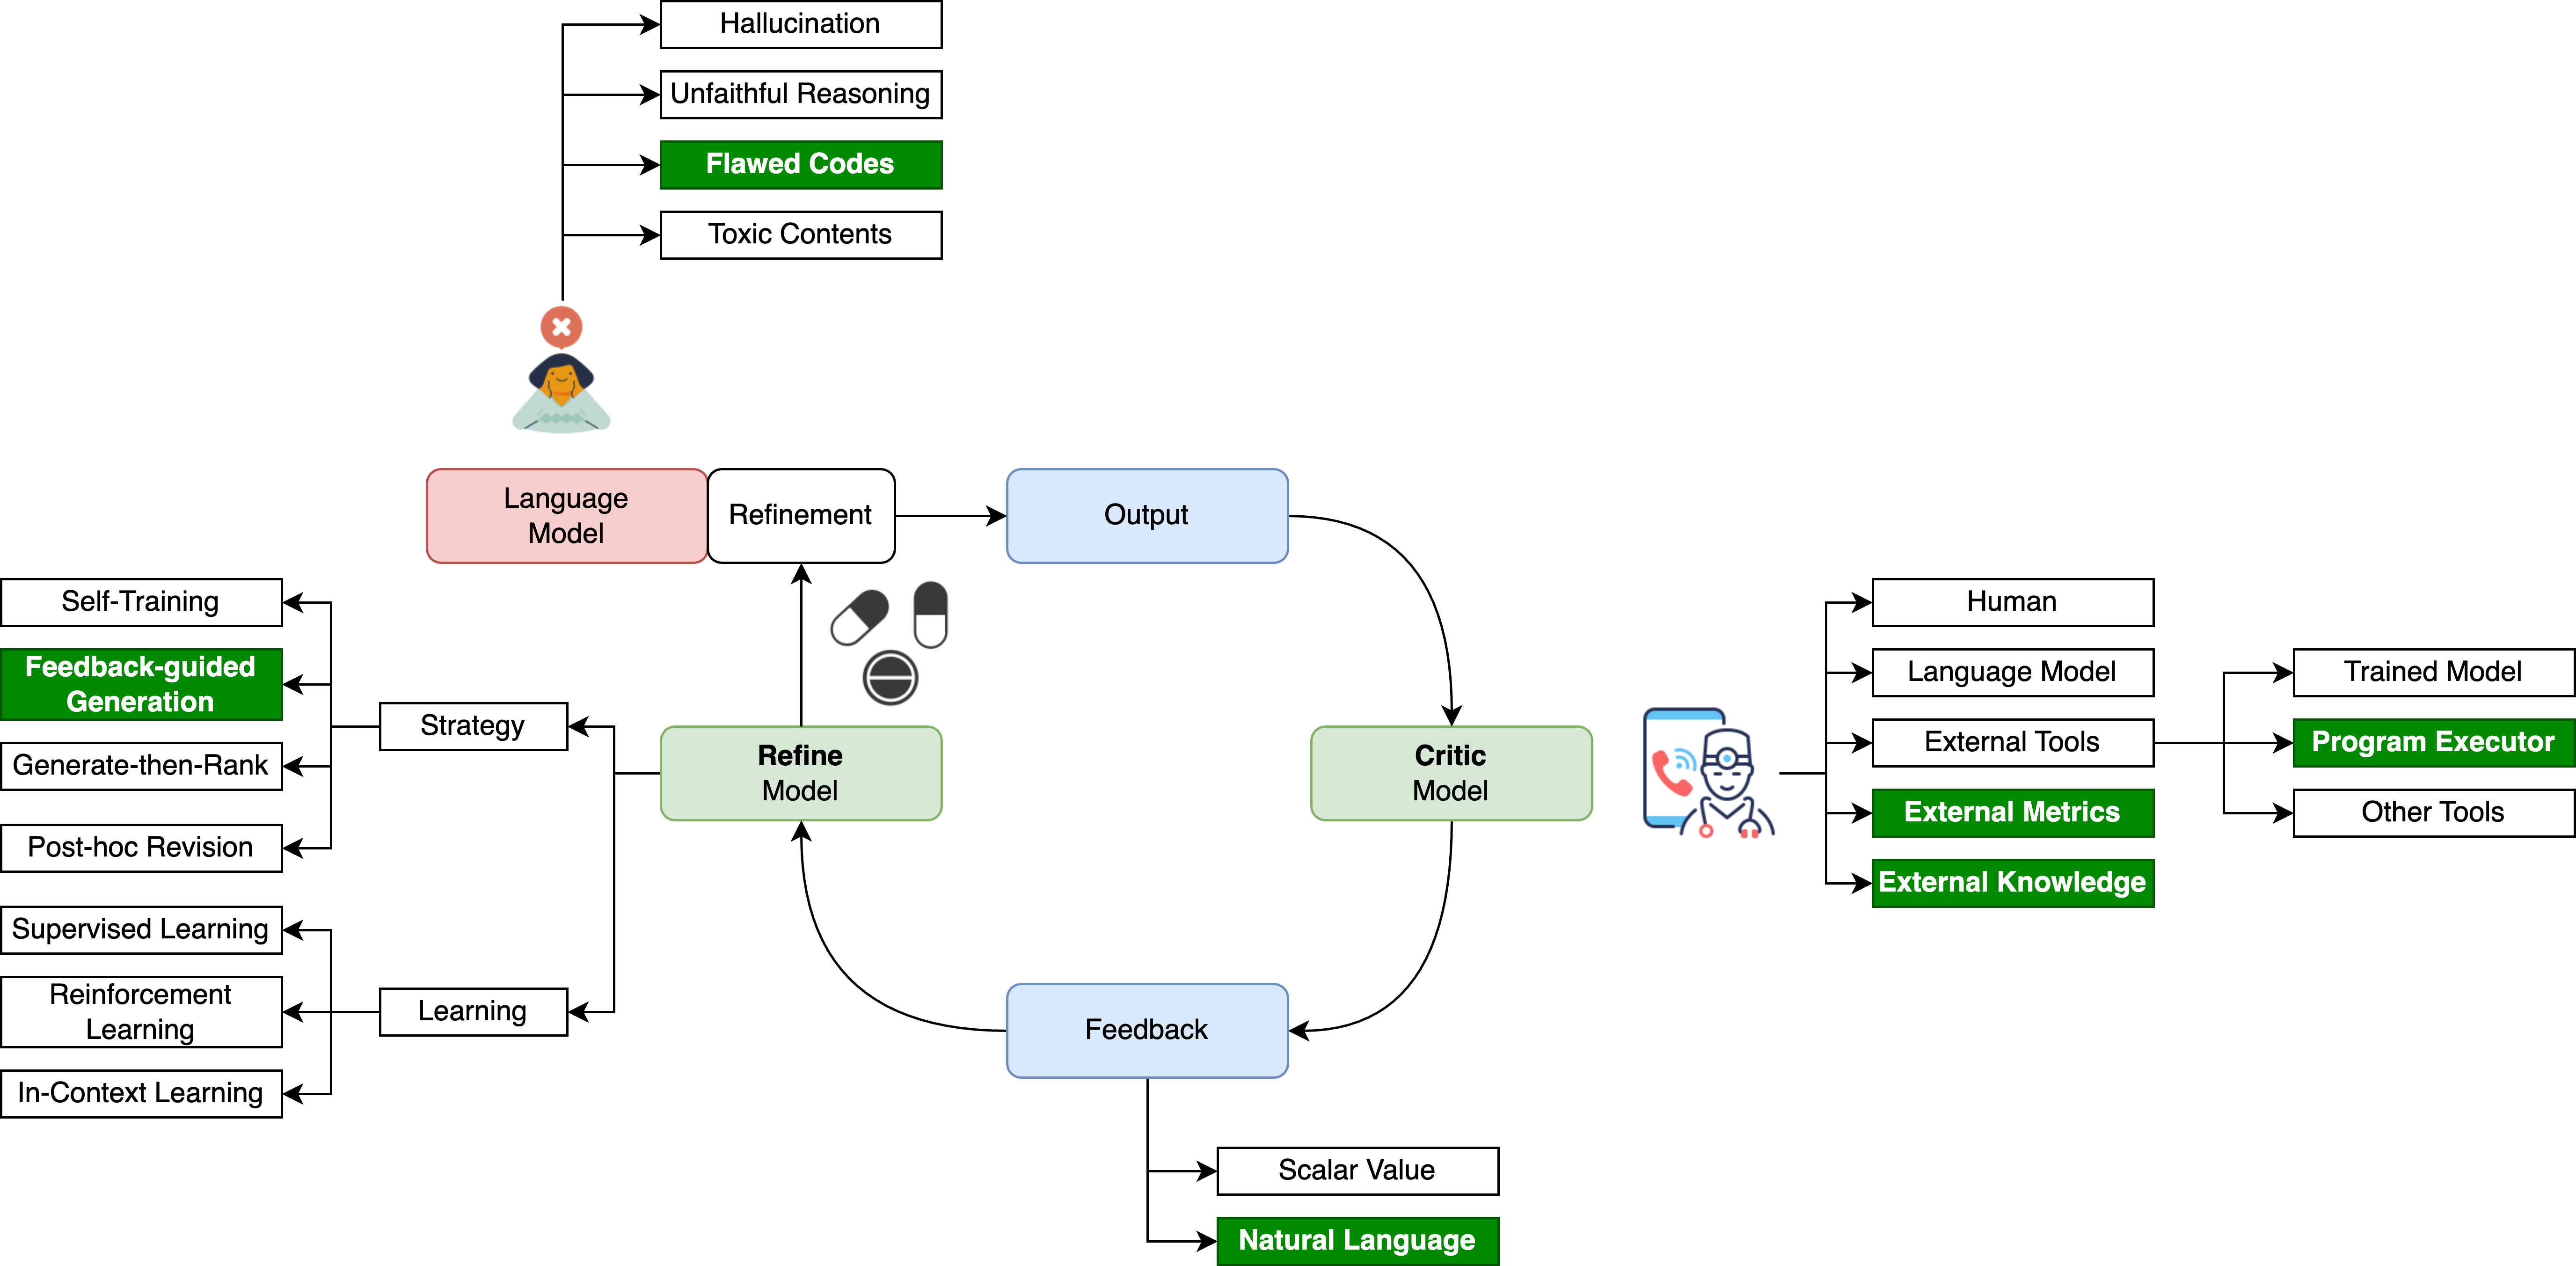
\includegraphics[width=0.90\textwidth]{img/direction_of_research.png}
    \caption{Focus areas of the current research.}\label{fig:direction_of_research}
\end{figure}

\chapter{Theoretical Background}
This section provides the relevant background to understand the fundamentals related to LLMs. Aligned with the objective of providing a comprehensive overview of this direction, this section offers a comprehensive yet concise outline of the basic concepts. The focus is more on the intuitive aspects and interested readers are referred to the original works for details.

\section{Tokenization}
LLMs are trained on text to predict text, and similar to other natural language processing systems, they use tokenization~\cite{webster1992tokenization} as the essential preprocessing step. It aims to parse the text into non-decomposing units called tokens. Tokens can be characters, subwords~\cite{kudo2018subword}, symbols~\cite{sennrich2015neural}, or words, depending on the size and type of the model. Some of the commonly used tokenization schemes in LLMs are briefed here. Readers are encouraged to refer to~\cite{mielke2021between} for a detailed survey.

\begin{enumerate}
    \item WordPiece~\cite{schuster2012japanese}: It was introduced in~\cite{schuster2012japanese} as a novel text segmentation technique for Japanese and Korean languages to improve the language model for voice search systems. WordPiece selects tokens that increase the likelihood of an n-grambased language model trained on the vocabulary composed of tokens.

    \item BPE~\cite{sennrich2015neural}: Byte Pair Encoding (BPE) has its origin in compression algorithms. It is an iterative process of generating tokens where pairs of adjacent symbols are replaced by a new symbol, and the occurrences of the most occurring symbols in the input text are merged.

    \item UnigramLM~\cite{kudo2018subword}: In this tokenization, a simple unigram LM is trained using an initial vocabulary of subword units. The vocabulary is pruned iteratively by removing the lowest probability items from the list, which are the worst performing on the unigram LM.
\end{enumerate}

\section{Attention in LLMs}
The attention mechanism computes a representation of the input sequences by relating different positions (tokens) of these sequences. There are various approaches to calculating and implementing attention, out of which some famous types are given below.

\begin{enumerate}
    \item \textbf{Self-Attention}~\cite{vaswani2017attention}: Self-attention, also known as intra-attention, connects all the sequence positions with $O(1)$ space complexity, which is highly desirable for learning long-range dependencies in the input. In self-attention, all the queries, keys, and values come from the same block (encoder or decoder).

    \item \textbf{Cross Attention}: In encoder-decoder architectures, the outputs of the encoder blocks act as the queries to the intermediate representation of the decoder, which provides the keys and values to calculate a representation of the decoder conditioned on the encoder. This attention is called cross-attention.

    \item \textbf{Full Attention}: The naive implementation of calculating self-attention is known as full attention.

    \item \textbf{Sparse Attention}~\cite{child2019generating}: Self-attention has a time complexity of $O(n^2)$, which becomes prohibitive when scaling the LLMs to large context windows. An approximation to self-attention was proposed in~\cite{child2019generating}, which greatly enhanced the capacity of GPT series LLMs to process a greater number of input tokens in a reasonable time.

    \item \textbf{Flash Attention}~\cite{dao2022flashattention}: The bottleneck for calculating attention using GPUs lies in memory access rather than computational speed. Flash Attention uses classical input tiling to process input blocks in GPU on-chip SRAM rather than doing IO for every token from the High Bandwidth Memory (HBM). An extension of this approach to sparse attention follows the speed gains of the full attention implementation. This trick allows even greater context-length windows in the LLMs as compared to those LLMs with sparse attention.
\end{enumerate}

\section{Encoding Positions}
The attention modules do not consider the order of processing by design. Transformer~\cite{vaswani2017attention} introduced `positional encodings' to feed information about the position of the tokens in input sequences. Several variants of positional encoding have been proposed~\cite{press2021train, su2024roformer}. Interestingly, a recent study [67] suggests that adding this information may not matter for the state-of-the-art decoder-only Transformers.

\begin{enumerate}
    \item \textbf{Absolute}: This is the most straightforward approach to adding the sequence order information by assigning a unique identifier to each position of the sequence before passing it to the attention module.

    \item \textbf{Relative}: To pass the information on the relative dependencies of different tokens appearing at different locations in the sequence, a relative positional encoding is calculated by some kind of learning. Two famous types of relative encodings are:
\end{enumerate}

Alibi~\cite{press2021train}: In this approach, a scalar bias is subtracted from the attention score calculated using two tokens which increases with the distance between the positions of the tokens. This learned approach effectively favors using recent tokens for attention.

RoPE~\cite{su2024roformer}: Keys, queries, and values are all vectors in the LLMs. RoPE involves the rotation of the query and key representations at an angle proportional to their absolute positions of the tokens in the input sequence. This step results in a relative positional encoding scheme which decays with the distance between the tokens.

\section{Activation Functions}
The activation functions serve a crucial role in the curvefitting abilities of the neural networks, as proved in~\cite{hornik1989multilayer}. The modern activation functions used in LLMs are different from the earlier squashing functions but are critical to the success of LLMs. The activation functions are discussed in this section.

\begin{enumerate}
    \item ReLU~\cite{nair2010rectified}: Rectified linear unit (ReLU) is defined as

    \begin{equation}
        ReLU(x)=\max(0, x).
    \end{equation}

    \item GeLU~\cite{hendrycks2016gaussian}: Gaussian Error Linear Unit (GeLU) is the combination of ReLU, dropout~\cite{srivastava2014dropout} and zoneout~\cite{krueger2016zoneout}. It is the most widely used activation function in contemporary LLMs literature.

    \item GLU variants~\cite{shazeer2020glu}: Gated Linear Unit~\cite{dauphin2017language} is a neural network layer that is an element-wise product $(\otimes)$ of a linear transformation and a sigmoid transformed $(\sigma)$ linear projection of the input given as

    \begin{equation}
        GLU(x, W, V, b, c)=(xW + b) \otimes \sigma(xV + c),
    \end{equation}

    where $X$ is the input of layer and $l, W, b, V$ and $c$ are learned parameters.

    GLU was modified in~\cite{shazeer2020glu} to evaluate the effect of different variations in the training and testing of transformers, resulting in better empirical results. Here are the different GLU variations introduced in~\cite{shazeer2020glu} and used in LLMs:

    \begin{equation}
        ReGLU(x, W, V, b, c) = \max (0, xW + b) \otimes,
    \end{equation}

    \begin{equation}
        GEGLU(x, W, V, b, c) = GELU(xW + b) \otimes(xV + c),
    \end{equation}

    \begin{equation}
        SwiGLU(x, W, V, b, c, \beta) = Swish \beta(xW + b) \otimes(xV + c).
    \end{equation}
\end{enumerate}

\section{Layer Normalization}
Layer normalization leads to faster convergence and is a widely used component in transformers. Different normalization techniques widely used in LLMs literature are provided in this section.

\begin{enumerate}
    \item LayerNorm: Layer norm computes statistics over all the hidden units in a layer $(l)$ as follows:

    \begin{equation}
        u^{l} = \frac{1}{n} \sum_{i}^{n} a_{i}^{l} \quad \sigma^{l} = \sqrt{\frac{1}{n} \sum_{i}^{n}{a_{i}^{l}-u^{l}}^{2}}
    \end{equation}

    where $n$ is the number of neurons in layer $l$ and $a_{i}^{l}$ is the summed input of neuron $i$ in layer $l$. LayerNorm provides invariance to rescaling of the weights and re-centering of the distribution.

    \item RMSNorm:~\cite{zhang2019root} proposed that the invariance properties of LayerNorm are spurious, and computationally efficient normalization achieving the same performance benefits as LayerNorm can be obtained by trading off re-centering invariance with speed. LayerNorm gives the normalized summed input to layer $l$ as follows:

    \begin{equation}
        \overline{a_{i}^{l}} = \frac{a_{i}^{l}-u^{l}}{\sigma} g_{i}^{l}
    \end{equation}

    where $g_{i}^{l}$ is the gain parameter. RMSNorm~\cite{zhang2019root} modifies $\overline{a_{i}^{l}}$ as:

    \begin{equation}
        \overline{a_{i}^{l}} = \frac{a_{i}^{l}}{\operatorname{RMS}\left(\mathbf{a}^{l}\right)} g_{i}^{l} \text {, where } \operatorname{RMS}\left(\mathbf{a}^{l}\right) = \sqrt{\frac{1}{n} \sum_{i}^{n}{a_{i}^{l}}^{2}}.
    \end{equation}

    \item Pre-Norm and Post-Norm: LLMs use the transformer~\cite{vaswani2017attention} architecture with some variations. The original implementation~\cite{vaswani2017attention} used layer normalization after the residual connection, commonly called post-LN, concerning the order of Multihead attention - Residual - LN. Another order of normalization, referred to as pre-LN~\cite{baevski2018adaptive}, places normalization before the self-attention layer as in LN - Multihead attention - Residual. Pre-LN is known to provide more stability in training~\cite{shleifer2021normformer}.

    \item DeepNorm: While pre-LN has certain benefits over post-LN training, pre-LN training has an unwanted effect on the gradients~\cite{shleifer2021normformer}. The earlier layers have larger gradients than those at the bottom. DeepNorm~\cite{wang2022deepnet} mitigates these adverse gradient effects. It is given as:

    \begin{equation}
        \mathbf{x}^{l_{f}} = LN\left(\alpha \mathbf{x}^{l_{p}}+G^{l_{p}}\left(\mathbf{x}^{l_{p}}, \theta^{l_{p}}\right)\right),
    \end{equation}

    where $\alpha$ is a constant and $\theta^{l_{p}}$ represents the parameters of layer $l_{p}$. These parameters are scaled by another constant $\beta$. Both constants depend only on the architecture.
\end{enumerate}

\section{Architectures}
Variants of the transformer architectures arising from differences in attention patterns and connection of transformer blocks are discussed here. Figure~\ref{fig:attention_patterns} illustrates the attention patterns of these architectures.

\begin{figure}[H]
    \centering
    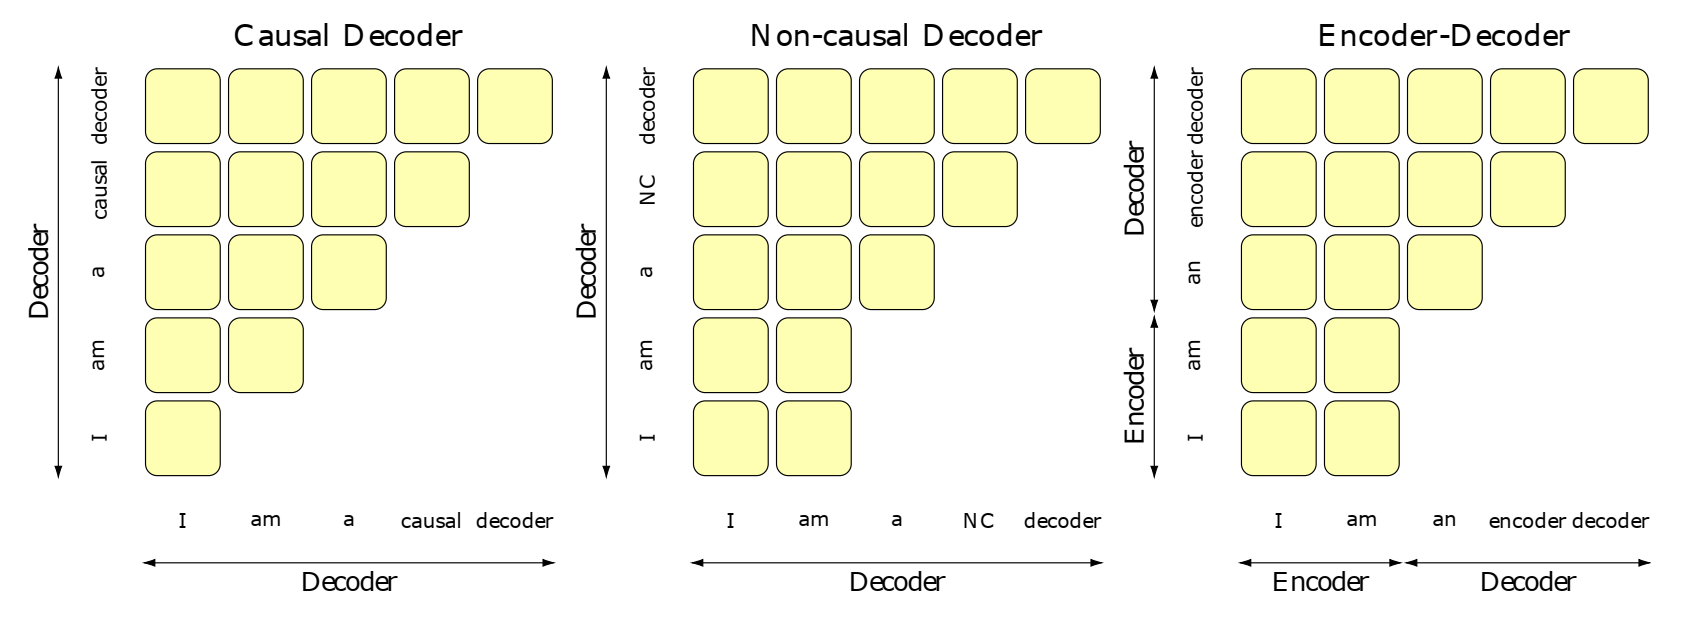
\includegraphics[width=0.8\textwidth]{img/attention_patterns.png}
    \caption{Attention patterns in a causal decoder, non-causal
    decoder, and encoder-decoder.~\cite{wang2022language}.}\label{fig:attention_patterns}
\end{figure}

\begin{enumerate}
    \item \textbf{Encoder Decoder}: Transformers were originally designed as sequence transduction models following prevalent model architectures for machine translation. They utilized an encoder-decoder architecture to train on human language translation tasks. This architecture is adopted by~\cite{raffel2020exploring, tay2022unifying}. In this scheme, an encoder encodes input sequences into variable length context vectors, which a decoder then processes to maximize a joint objective of minimizing the gap between predicted token labels and actual target token labels.

    \item \textbf{Causal Decoder}: The underlying objective of an LLMs is to predict the next token based on the input sequence. Although additional encoder information strongly binds the prediction to context, in practice LLMs can perform well lacking an encoder~\cite{liu2018generating}, relying solely on the decoder. Like the original encoder-decoder's decoder block, this decoder restricts backward information flow, i.e. predicted token $t_k$ depends only on preceding tokens up to $t_{k-1}$. This is the most widely used variant in state-of-the-art LLMs.

    \item \textbf{Prefix Decoder}: The causally masked attention is reasonable in encoder-decoder architectures where the encoder can attend to all sentence tokens from every position via self-attention. This means the encoder can also attend to tokens $t_{k+1}$ to $t_n$ in addition to $t_1$ to $t_{k-1}$ when calculating the representation for $t_k$. But dropping the encoder also loses this attention flexibility. A decoder-only architecture variation changes the mask from strictly causal to fully visible on a portion of the input. The prefix decoder is also known as a non-causal decoder architecture.
\end{enumerate}

\section{Model Adaptation}
LLMs adaptation stage fundamentals, from pre-training to fine-tuning for downstream tasks and utilization, are discussed here.

\begin{enumerate}
    \item Pre-Training: Initially, the model is trained self-supervised on a large corpus to predict next tokens given the input. LLMs design choices vary for architectures, building blocks, and loss functions.

    \item Fine-Tuning: There are different LLMs fine-tuning approaches, briefly discussed here.
\end{enumerate}

\textbf{Transfer Learning}: Pre-trained LLMs perform well for various tasks~\cite{brown2020language, chowdhery2023palm}. But to improve performance for a downstream task, pre-trained models are fine-tuned with task-specific data~\cite{raffel2020exploring, xue2020mt5}, known as transfer learning.

\textbf{Instruction-tuning}: To enable effective model response to user queries, the pre-trained model is fine-tuned on instruction formatted data, i.e. an instruction and input-output pair. Instructions generally comprise multi-task data in plain natural language, guiding the model to respond according to the prompt and input. This fine-tuning improves zero-shot generalization and downstream task performance. Details on instruction data formatting and styles are available in~\cite{chung2022scaling, zhao2023survey, iyer2022opt}.

\textbf{Alignment-tuning}: LLMs are prone to generate false, biased, and harmful text. To develop helpful, honest, and harmless models, alignment with human feedback is used. Alignment involves asking LLMs to generate unexpected responses, then updating parameters to avoid such responses~\cite{ouyang2022training, touvron2023llama, sun2023principle}. This ensures LLMs operate according to human intentions and values. A model is considered `aligned' if it meets the three criteria of being helpful, honest, and harmless or `HHH'~\cite{askell2021general}.

Researchers employ reinforcement learning with human feedback~\cite{ziegler2019fine} for model alignment. In RLHF, a fine-tuned model on demonstrations is further trained with reward modeling (RM) and reinforcement learning (RL). RM and RL pipelines in RLHF are briefly discussed below.

Reward modeling trains a model to rank generated responses by human preferences using a classification objective. To train the classifier, humans annotate LLMs generated responses based on HHH criteria.

Reinforcement learning combines the reward model for alignment in the next stage. The trained reward model ranks LLM-generated responses into preferred vs. dispreferred, which alignment uses via proximal policy optimization (PPO). This process repeats iteratively until convergence.

\begin{enumerate}
    \setcounter{enumi}{2}
    \item Prompting/Utilization: Prompting queries trained LLMs to generate responses. LLMs can be prompted in various setups, either adapting to instructions without fine-tuning or with fine-tuning containing different prompt styles~\cite{chung2022scaling, kim2023cot, liu2023zero}. A good prompt engineering guide is available at~\cite{saravia2022prompt}. Various widely used prompt setups are discussed below.
\end{enumerate}

\textbf{Zero-Shot Prompting}: LLMs are zero-shot learners and capable of answering queries never seen before. This prompting style requires LLMs to answer user questions without any examples in the prompt.

\textbf{In-context Learning}: Also known as few-shot learning, here multiple input-output demonstration pairs are provided to the model to generate the desired response. This adaptation style is also called few-shot learning. Discussions on formatting in-context learning (ICL) templates are available in~\cite{dong2022survey, zhao2023survey, wang2022super, chung2022scaling}.

\textbf{Reasoning in LLMs}: LLMs are zero-shot reasoners and can be provoked to generate answers to logical problems, task planning, critical thinking, etc. with reasoning. Generating reasons is only possible using different prompting styles, while to further improve LLMs on reasoning tasks many methods~\cite{chung2022scaling, iyer2022opt} train them on reasoning datasets. Various prompting techniques for reasoning are discussed below.

\textbf{Chain-of-Thought}: A special prompting case where demonstrations contain reasoning information aggregated with inputs and outputs so the model generates outcomes with step-by-step reasoning. More CoT prompt details are in~\cite{huang2022towards, wei2022chain, kim2023cot}.

\textbf{Self-Consistency}: Improves CoT performance by generating multiple responses and selecting the most frequent answer~\cite{wang2022self}.

\textbf{Tree-of-Thought}: Explores multiple reasoning paths with possibilities to look ahead and backtrack for problem-solving~\cite{yao2023tree}.

\textbf{Single-Turn Instructions}: In this prompting setup, LLMs are queried only once with all relevant information in the prompt. LLMs generate responses by understanding the context either zero-shot or few-shot.

\textbf{Multi-Turn Instructions}: Solving complex tasks requires multiple LLMs interactions, where feedback and responses from other tools are next round LLMs inputs. This style of using LLMs in the loop is common in autonomous agents.

\chapter{Referenced Works}
This section discusses two major works referenced in this thesis: the Chain-of-Thought framework for facilitating reasoning in language models, and a modular code analysis framework for improving code generation. Both claim state-of-the-art results in their domains. Their key ideas, results, and potential for further improvement are examined.

\section{CoT Prompting}
Humans often solve complex reasoning tasks by decomposing them into intermediate steps. For example, when solving multi-step math word problems, people break the problem down into smaller steps, solving each sub-problem sequentially. The CoT paper aims to enable language models to mimic this reasoning process by generating coherent chains of thought.

The authors demonstrate that with the right few-shot prompting, large language models can produce chains of thought leading to correct solutions for problems they initially failed. As shown in Figure~\ref{fig:cot_prompting}, a model generates a step-by-step reasoning chain to solve a math problem it previously answered incorrectly. Although resembling a solution, these reasoning chains are called chains of thought to emphasize they mimic human step-by-step reasoning.

\begin{figure}[H]
    \centering
    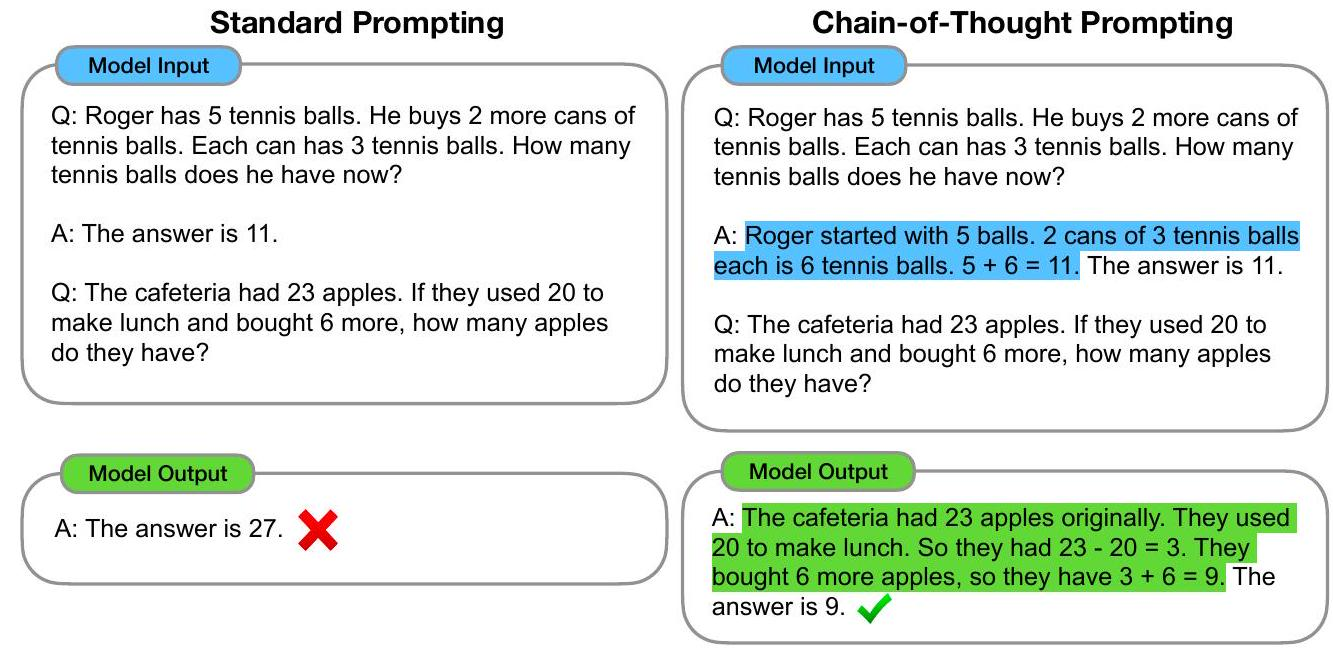
\includegraphics[width=0.8\textwidth]{img/cot_prompting.jpg}
    \caption{Example of CoT reasoning processes.~\cite{wei2023chainofthought}.}\label{fig:cot_prompting}
\end{figure}

Chain-of-thought prompting has several key advantages:

\begin{enumerate}
    \item It allows dynamic computation allocation, with more steps for harder problems needing more reasoning.
    \item It provides interpretability into model reasoning, aiding debugging.
    \item It is widely applicable to language-based reasoning tasks.
    \item It only requires including reasoning chain examples in few-shot prompts.
\end{enumerate}

In summary, chain-of-thought prompting is a promising approach to improve reasoning and interpretability in language models.

\section{Modular Code Analysis}
Experienced programmers solve problems by decomposing them into modular sub-tasks and iteratively refining solutions. The modular code analysis paper proposes CodeChain~\cite{le2023codechain}, which mimics this process to improve code generation in language models.

Specifically, CodeChain first elicits modular solutions using chain-of-thought prompting. It then recursively revises generated code by conditioning on representative sub-module code snippets sampled from previous outputs. This iterative refinement with reusable code `legs up' future generations.

Experiments demonstrate CodeChain significantly improves performance on challenging benchmarks like APPS~\cite{hendrycks2021measuring} and CodeContests~\cite{Li_2022}, achieving state-of-the-art results. For example, on APPS it increases pass@1 by over 35\% on average. Ablations provide insights into the drivers of CodeChain's effectiveness.

In summary, CodeChain is a novel way to incorporate modularity and iterative refinement to boost code generation in language models, inspired by experienced programmers' problem solving process. The gains on benchmark datasets are promising.

\section{Evaluation Results}
On the APPS benchmark, CodeChain with GPT-3.5 and WizardCoder~\cite{luo2023wizardcoder} models achieves new state-of-the-art pass@1 results. With test case filtering, CodeChain+GPT-3.5 further improves to over 35\% average pass@1 across difficulty levels. This demonstrates the efficacy of CodeChain's iterative refinement approach on challenging code generation tasks.

\begin{table}[H]
    \caption{APPS test results: results with $\dagger$ are for models finetuned on APPS training data. Performance by pass@ 1 (\%)}\label{tab:apps_results}
    \begin{center}
        \begin{tabular}{lccccc}
            \hline
            Model & Size & Introductory & Interview & Competition & All \\
            \hline
            Codex & 12B & 4.14 & 0.14 & 0.02 & 0.92 \\
            CodeT5 $\dagger$ & 770M & 6.60 & 1.03 & 0.30 & 2.00 \\
            CodeRL+CodeT5 $\dagger$ & 770M & 7.08 & 1.86 & 0.75 & 2.69 \\
            text-davinci-002 & - & - & - & - & 7.48 \\
            Self-edit+text-davinci-002 & - & - & - & - & 7.94 \\
            code-davinci-002 & - & 29.30 & 6.40 & 2.50 & 10.20 \\
            \hline
            WizardCoder & 15B & 26.04 & 4.21 & 0.81 & 7.90 \\
            CodeChain+WizardCoder & 15B & 26.29 & 7.49 & 3.75 & 10.50 \\
            \hline
            GPT3.5 & - & 48.00 & 19.42 & 5.42 & 22.33 \\
            CodeChain+GPT3.5 & - & $\mathbf{5 4 . 5 0}$ & $\mathbf{2 8 . 1 1}$ & $\mathbf{1 2 . 3 8}$ & $\mathbf{3 0 . 2 4}$ \\
            \hline
        \end{tabular}
    \end{center}
\end{table}

\section{Conclusion}
While the CodeChain framework has achieved strong results on competitive programming benchmarks, there are opportunities to improve its applicability to real-world tasks:

\begin{enumerate}
    \item CodeChain has focused on synthetic competitive programming problems, which may not translate to performance on real-world code generation.

    \item The modular analysis in CodeChain concentrates on code generation alone, without considering dependencies on external libraries. However, bugs in real applications often arise from misalignments between code logic and library usage.
\end{enumerate}

This research aims to enhance CodeChain by incorporating modular analysis of code logic alongside library dependencies. The goal is to build external knowledge sources that language models can reference in a modular, targeted way when generating code.

Additionally, this work shifts the evaluation domain from competitive programming to more practical data science tasks, using the DS-1000~\cite{pmlr-v202-lai23b} benchmark. DS-1000 contains 1,000 diverse, real-world data science problems from StackOverflow spanning multiple Python libraries. It has high-fidelity automatic evaluation, ensuring functional correctness and appropriate API usage. Problem statements are modified from the original posts to prevent memorization. The best current model, Codex-002~\cite{madaan2022language}, achieves only 43.3\% accuracy, providing ample room for improvement.

In summary, this research proposes to augment CodeChain with logic/library modularity and demonstrate gains on practical data science problems. By tackling real-world tasks and dependencies, the enhanced framework could better support applied code generation compared to solely tackling competitive programming.

\chapter{Tentative Plan}

\chapter{Tentative Research Contents}

\chapter{Conclusion}

\newpage
\renewcommand{\bibname}{References}
\bibliography{references}

\end{document}
